\chapter{Neutron Analysis} \label{ch:neutrons}

As mentioned in chapter 4, the MuSun experiment includes a set of eight auxiliary neutron detectors in addition to the primary electron detector array. 
Although decay electrons are easier to detect and permit a more precise extraction of the muon capture rate, direct detection of neutrons remains a valuable tool. 
The neutron detectors are useful for three main analyses:
\begin{itemize}
  \item Monitoring the muon kinetics and constraining kinetic fit parameters.
  \item Measuring wall stop contamination and determining the lifetime correction.
  \item Estimating the ratio of the quartet and doublet capture rates in deuterium.
\end{itemize}

\section{Neutron Sources}

The MuSun neutron detectors are useful for so many analyses because they can observe a large variety of different signals.
Figure \ref{fig:kinetics_chart} highlights all the sources of neutrons related to muon kinetics in the target.
There are also neutrons produced by the beam and by scattering events, which are not included in the chart.
In total, we identify five major neutron sources of interest.

\begin{figure}[h]
  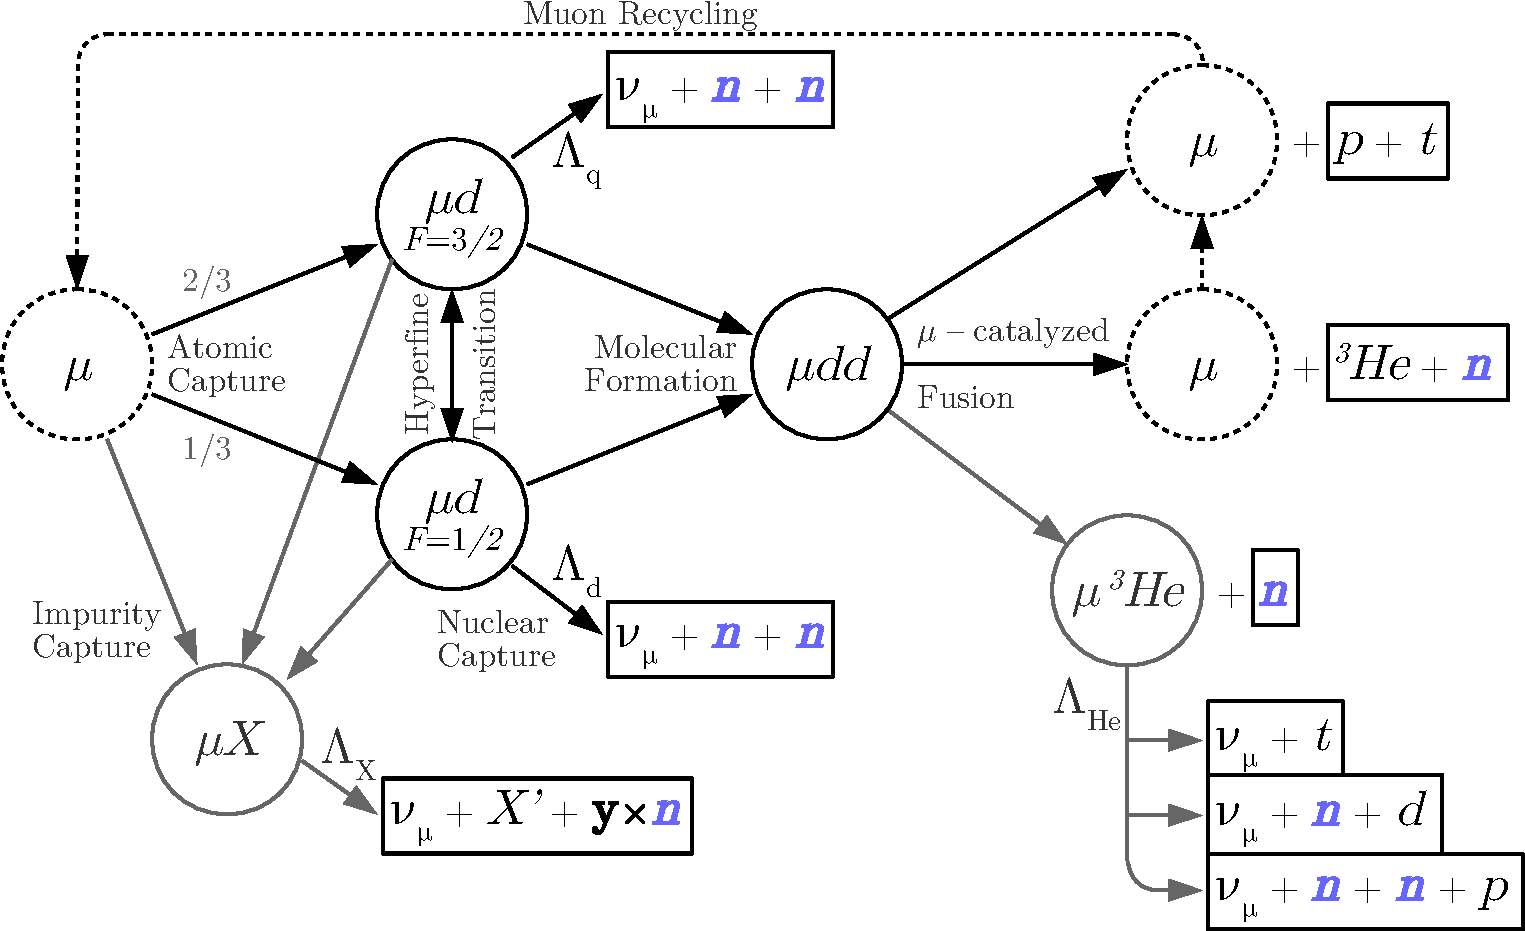
\includegraphics[width=\textwidth]{neutrons/figures/kinetics_neutrons_highlighted-crop.pdf}
  \caption{Full muon kinetics in $D_2$ gas. Neutron emissions are highlighted in blue.}
  \label{fig:kinetics_chart}
\end{figure}

\subsection{Muon Capture in Deuterium}

First, there are of course the neutrons produced by nuclear muon capture in deuterium.
As mentioned previously, we could attempt to directly measure the capture rate using these neutrons, albeit with lower accuracy than the lifetime method.
A more interesting possibility is to study the time dependence of the signal which can constrain the ratio of the quartet and doublet state capture rates.

The time dependence of the deuterium capture rate depends on the muon kinetics, shown in figure \ref{fig:kinetics_chart}.
The kinetics have already been discussed in section ?, so we will not go into great detail here.
%todo - ref
Capture may occur in both of the deuterium hyperfine states, but at significantly different rates.
For the doublet state, we expect a rate of $\Lambda_d \approx 400 s^{-1}$, compared to $\Lambda_q \approx 10 s^{-1}$ for the quartet state. 
Muon capture on deuterium produces a pair of neutrons, so the expected total neutron signal is:
\begin{equation}
2[\Lambda_d N_d(t) + \Lambda_q N_q(t)].
\end{equation}
Because the MuSun operating conditions are optimized to rapidly deplete the quartet state, the neutron signal increases at early times as the muons transfer to the doublet state.
After the quartet state is depleted the neutron signal transitions to a slower exponential decay following the muon lifetime, as seen in figure \ref{fig:shape_capture}.

\begin{figure}[h]
  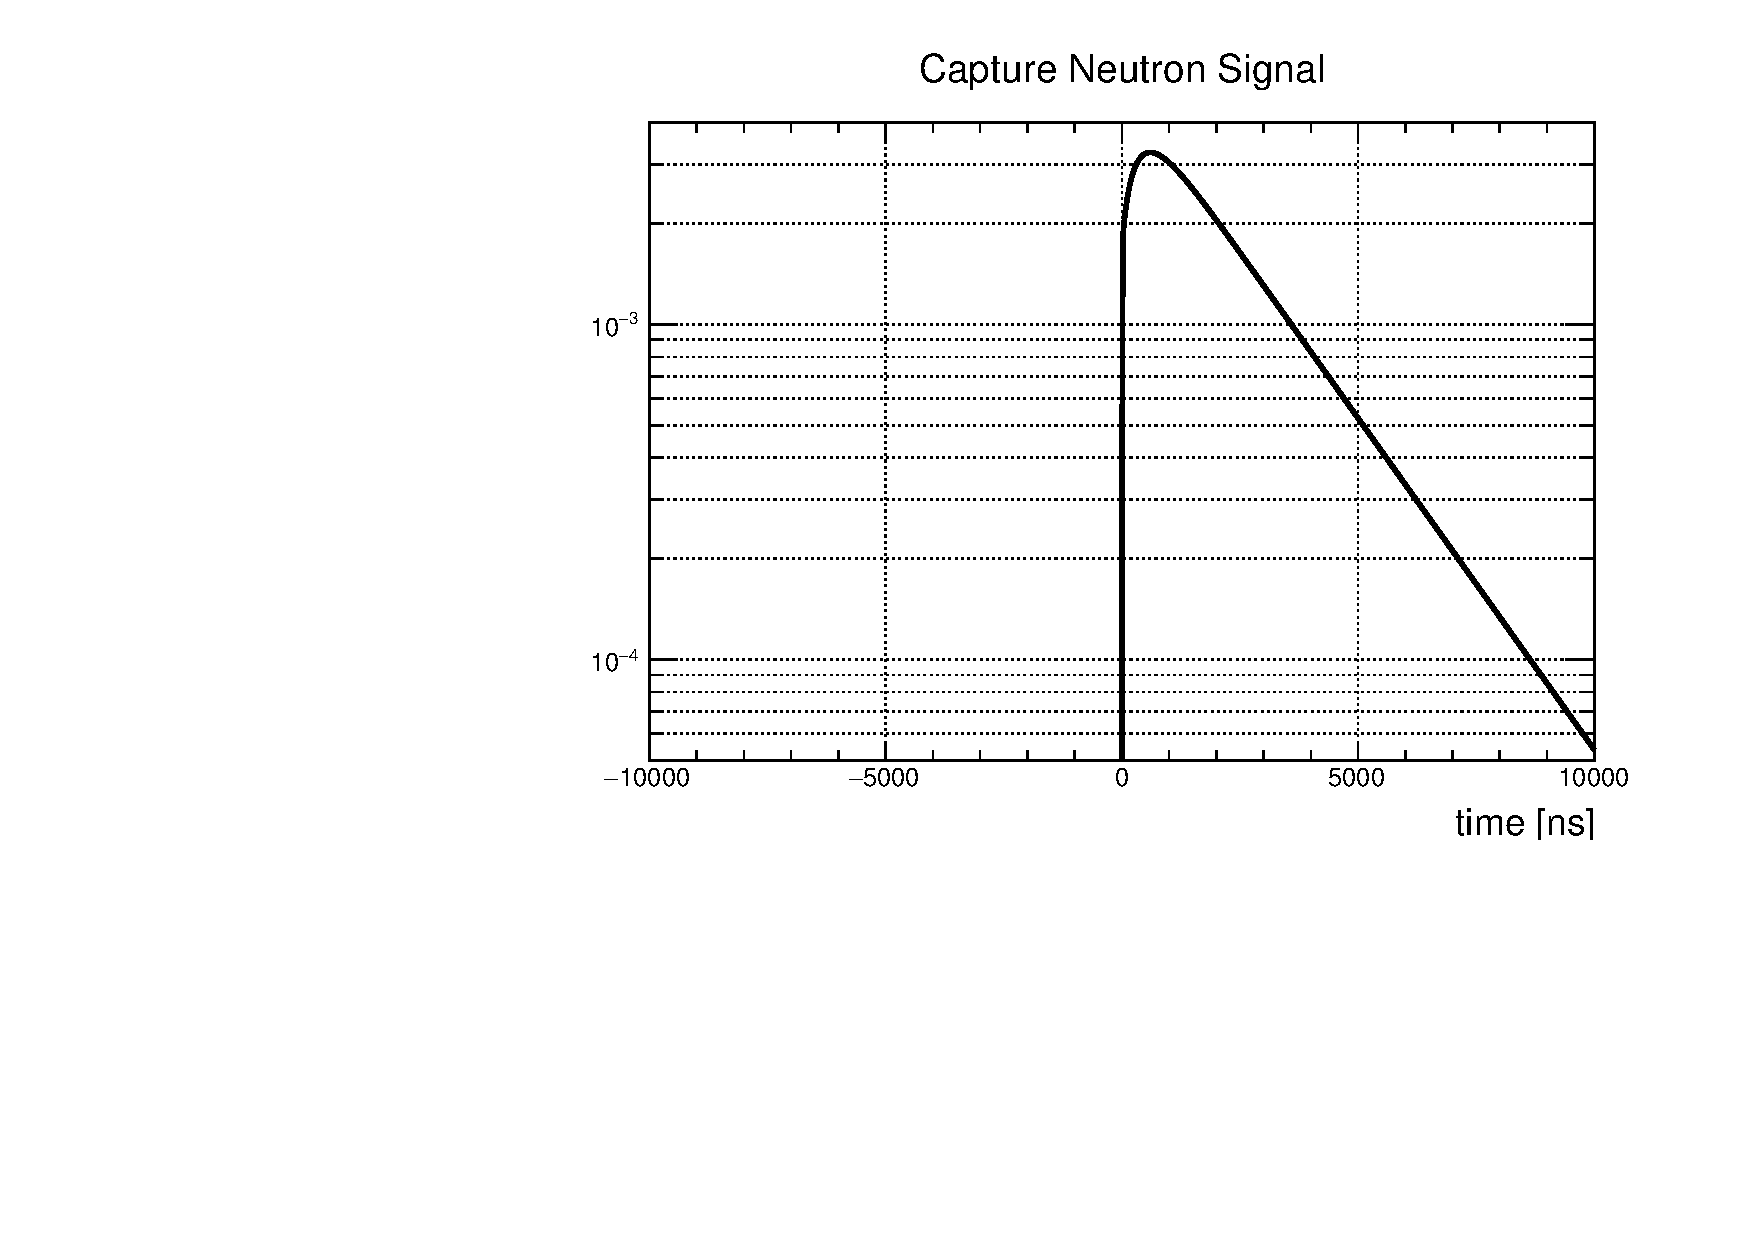
\includegraphics[width=\textwidth]{neutrons/figures/shape_capture.pdf}
  \caption{Expected deuterium capture neutron time distribution due to muon kinetics.}
  \label{fig:shape_capture}
\end{figure}

Because muon capture and muon decay both convert the muon into a neutrino, the two reactions are mutually exclusive.  
Thus, a muon capture event is characterized by the lack of any decay electron. 
However, the 70\% solid angle coverage of the electron detectors limits the effectiveness of an electron veto.
Capture events could in principle be identified cleanly by searching for the pair of coincident capture neutrons, but the efficiency of the MuSun neutron detectors is too low for this to be practical.
Muon capture on deuterium involves a three body final state, yielding neutrons with a continuous energy distribution that peaks around 1.5 MeV but extends as high as 50 MeV. 

\subsection{Muon Catalyzed Fusion}

Muons in deuterium also undergo muon catalyzed fusion, and in the case of $^3He$ fusion a neutron is produced.  
The fusion signal is related to the hyperfine states in the same way as the capture signal, except now the neutrons are produced according to the fusion rates:
\begin{equation}
\beta[\lambda_d N_d(t) + \lambda_q N_q(t)].
\end{equation}
The doublet fusion rate is $\lambda_d = 0.053(3) \mu s^{-1} * \phi$, while the quartet fusion rate is much higher at $\lambda_q = 3.98(5) \mu s^{-1} * \phi$.
Here $\beta = 0.517(15)$ is the $^3He$ fusion fraction and $\phi \approx 5\%$ is the pressure relative to liquid deuterium.
The high quartet fusion rate means that instead of a buildup at early times we now have a signal that starts out very large and rapidly decays.

\begin{figure}[h]
  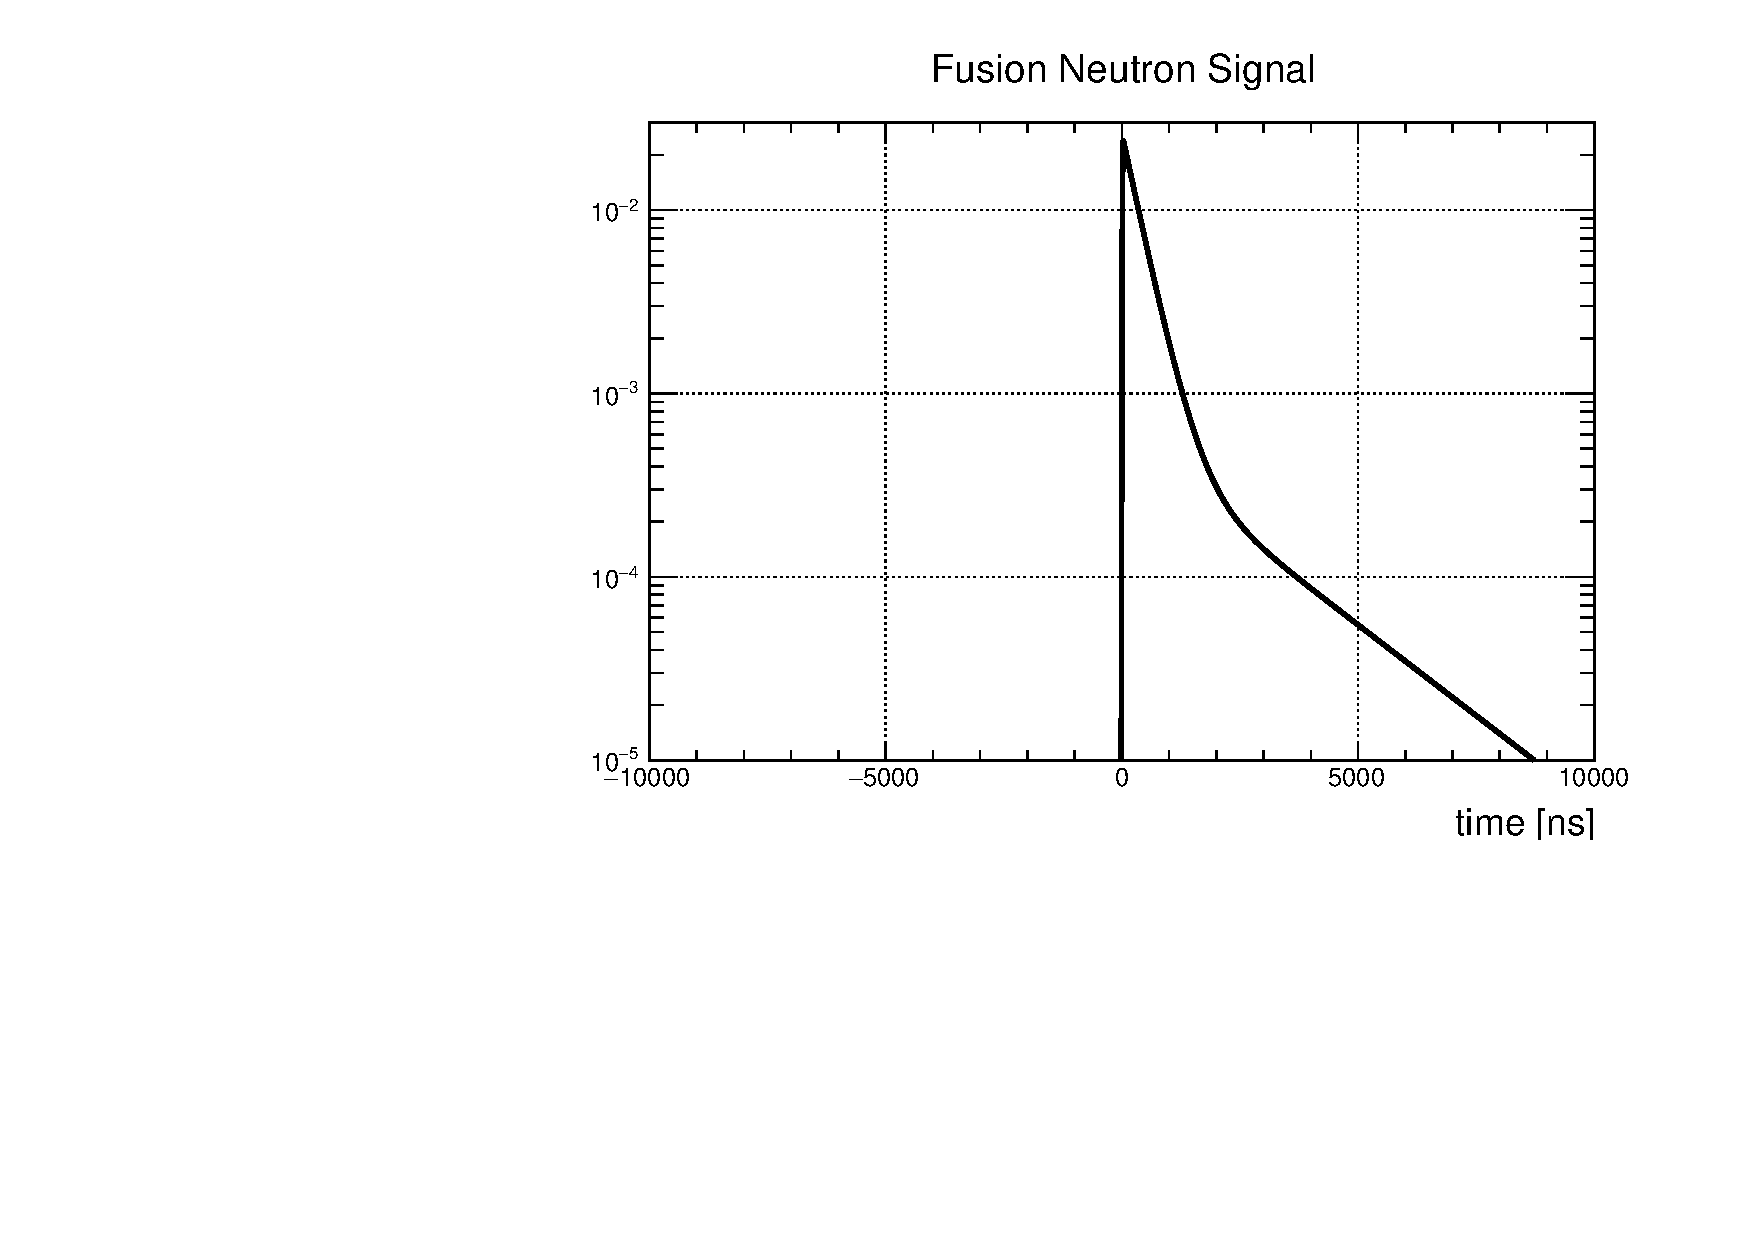
\includegraphics[width=\textwidth]{neutrons/figures/shape_fusion.pdf}
  \caption{Expected deuterium $^3He$ fusion neutron time distribution due to muon kinetics.}
  \label{fig:shape_fusion}
\end{figure}

Muon catalyzed fusion events are uniquely characterized by additional energy deposition in the TPC due to fusion products.  
For p-t fusions this energy deposition is large, and in S-energy plots it produces a peak with well-separated from non-fusion events as seen in figure \ref{fig:cuts_svt}.
However, $^3He$ deposits much less energy and the events are not cleanly separated from normal muon stops.  
To improve our ability to distinguish these events, I also define a quantity called T-Energy from the E9 and fusion energies.
Two dimensional cuts are then defined in S-T space, as shown in figure \ref{fig:cuts_svt}.
A pair of cuts are defined, one to identify fusions and one to identify captures.
The region where the distributions overlap is usually rejected in either case.
These are similar to cuts in E0-E1 space for normal stops, but can treat stops with extra TPC clusters somewhat differently.

%todo - add neutron selected plot for comparison, maybe just use E0 vs E1 for clarity
\begin{figure}[h]
  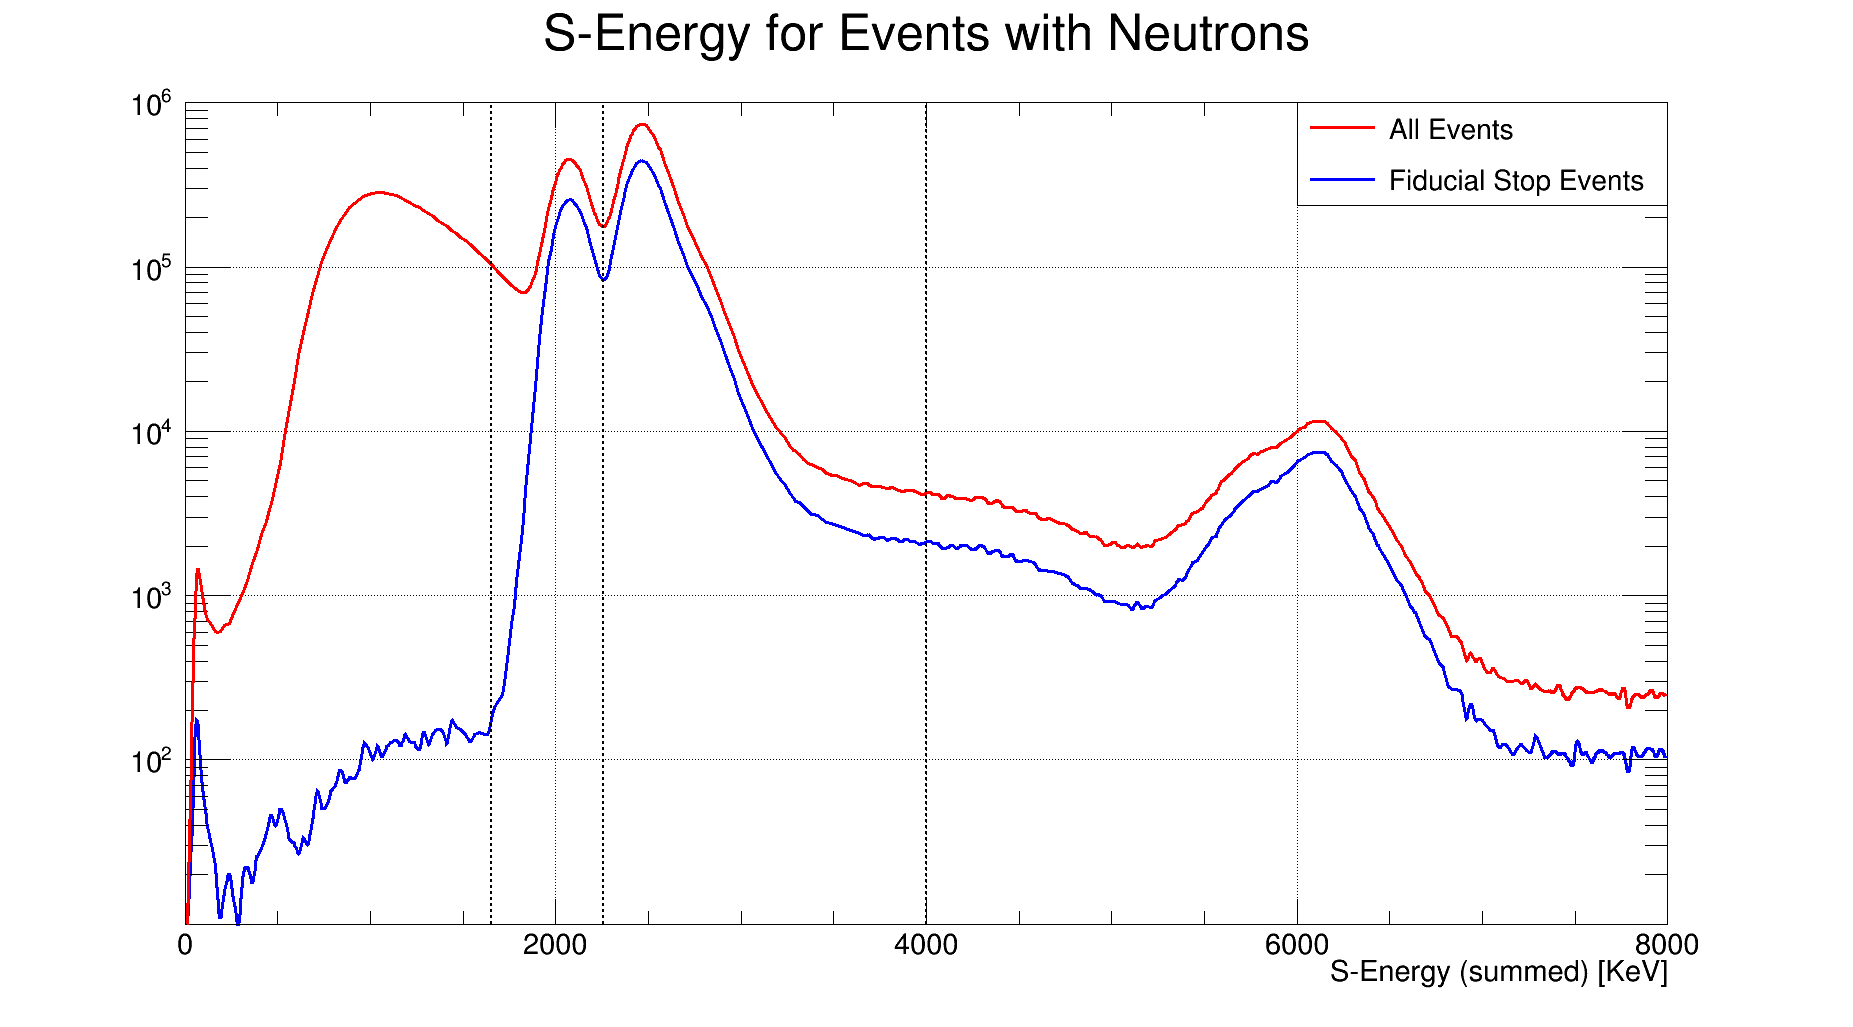
\includegraphics[width=0.49\textwidth]{neutrons/figures/Cuts_SEnergy.png}
  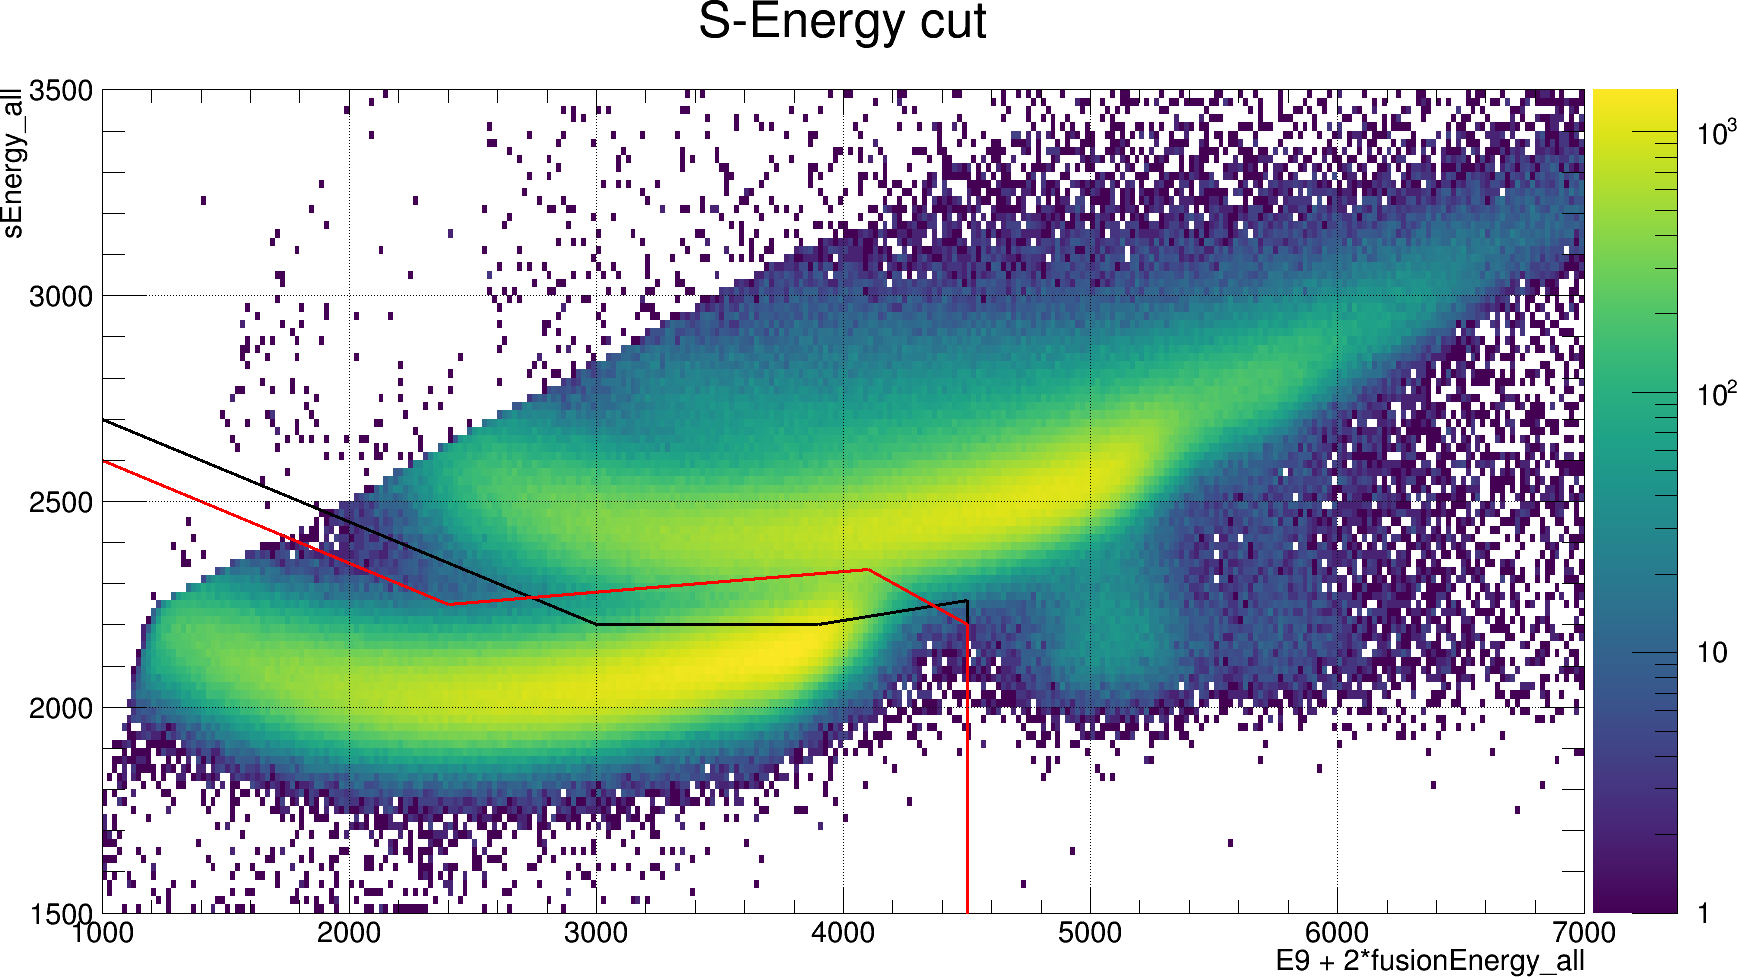
\includegraphics[width=0.49\textwidth]{neutrons/figures/Cuts_SEnergyVsTEnergy.png}
  \caption{Left: 1D S-energy plot for neutron events, with and without a fiducial cut.  Right: 2D cuts defined based on S- and T-energy.  The black line is defined based on the fusion distribution, while the red is defined based on the captures.}
  \label{fig:cuts_svt}
\end{figure}

Muon catalyzed fusion is non-destructive to the muon, so most fusion events are followed by an electron from the subsequent decay of the muon.
These delayed electrons form a fairly distinctive signal, but such a cut has complicated effects on the backgrounds so it is not advisable.
The sticking probability for $^3He$ fusions is 12\%, and stuck muons may capture on the $^3He$ potentially producing one or two additional neutrons. 
The remaining 88\% of $^3He$ fusions produce a free muon, which is recycled and has the possibility of catalyzing one or more additional fusion reactions before decaying.
Multiple fusions and $^3He$ capture are both quite rare, and are currently neglected in the neutron analysis.

Because the muon does not participate directly in muon catalyzed fusion, there is essentially a two body final state.
This means that energy and momentum conservation can only be satisfied by mono-energetic neutrons at 2.45 MeV. 
The energy deposition in the detector can be anything smaller than the total neutron energy, due to variation in the scattering angle, and the observed energy distribution is seen in figure \ref{fig:fusion_energy}.
Although the fusion neutrons cannot be cleanly selected with an energy cut, they can at least be suppressed by selecting neutrons with energies above 2.45 MeV. 

\begin{figure}[h]
  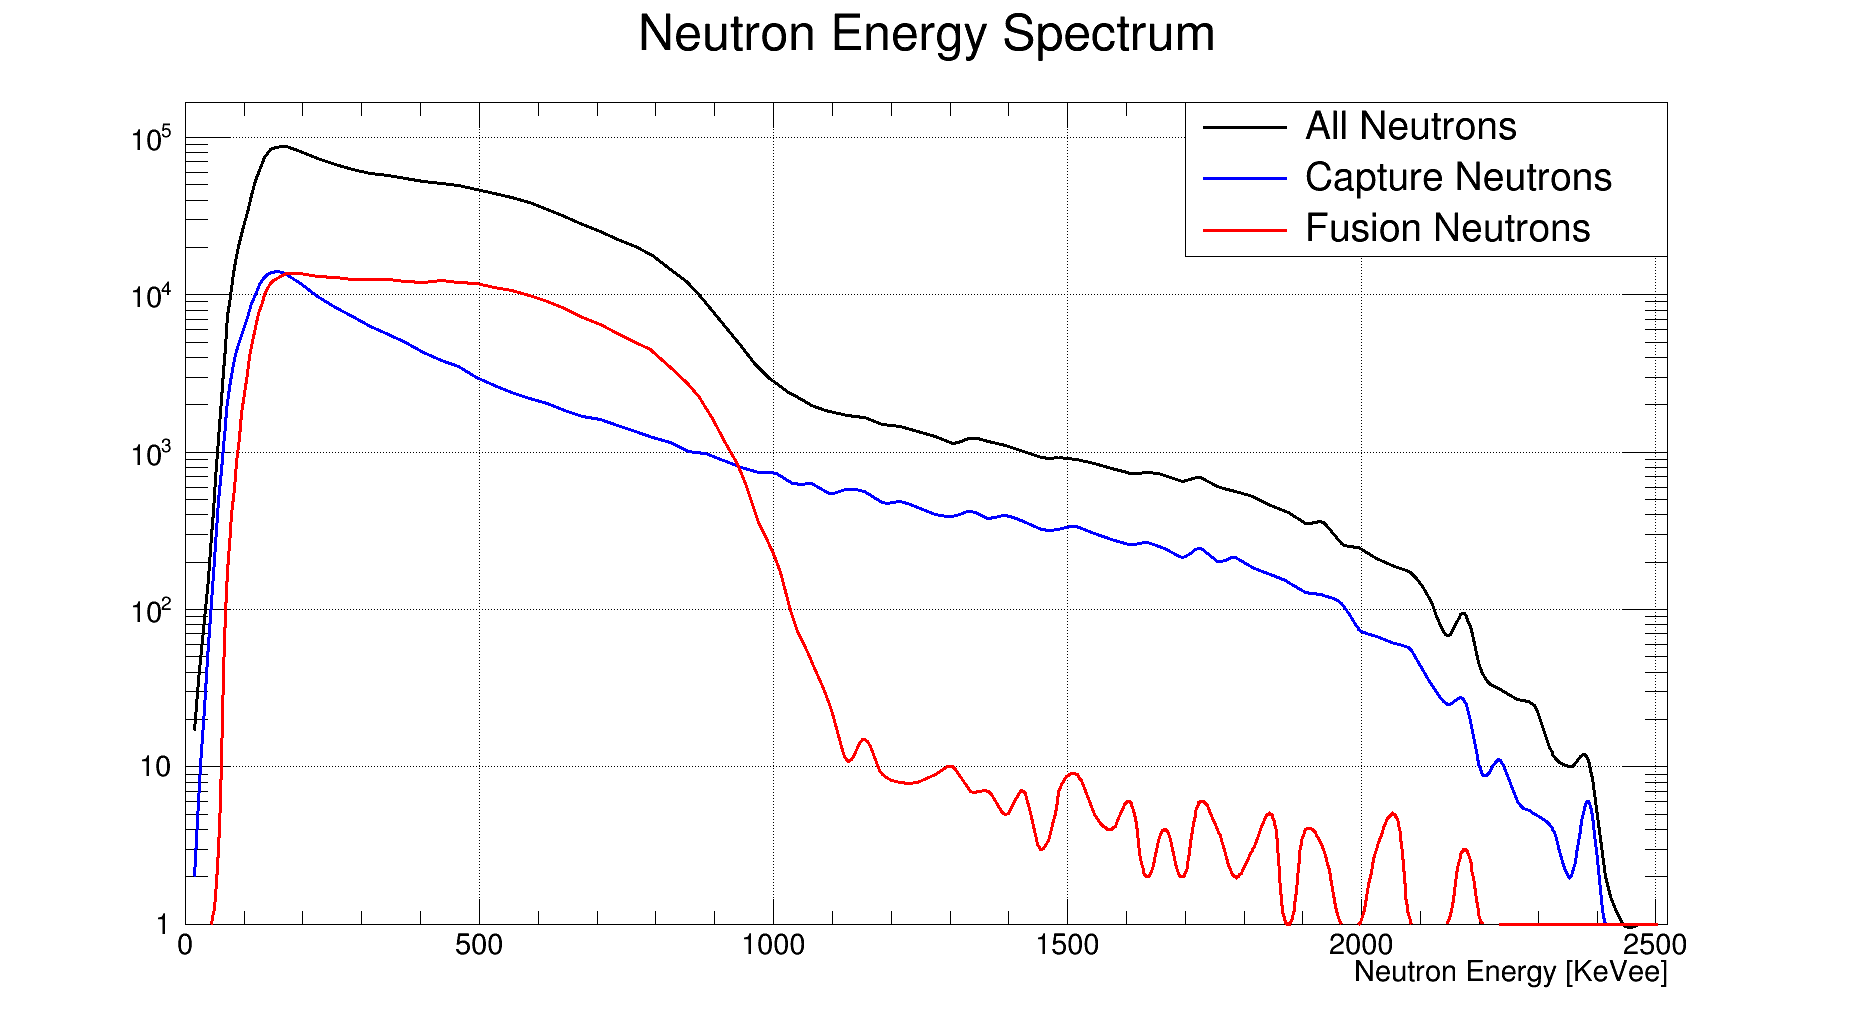
\includegraphics[width=\textwidth]{neutrons/figures/NeutronEnergy.png}
  \caption{Comparison of observed fusion and capture neutron energies.}
  \label{fig:fusion_energy}
\end{figure}

While I currently only model a single fusion reaction per event, it is worth noting that the TPC energy and the neutron energy cuts have different effects on events with both fusion and capture.
Using the TPC energy to eliminate fusions will cut both the fusion neutrons and any subsequent capture neutrons.  
Cutting on the neutron energy will only remove the fusion neutrons themselves, and leave the following capture neutrons intact.
This can be seen in figure \ref{fig:fusion_energy}, where the "fusion" distribution includes a small high-energy tail due to these captures.

\subsection{Muon Capture on Other Materials}

Recall that the rate of nuclear muon capture is proportional to $Z^4$ for the capturing material. 
Because the rate that neutrons are emitted is directly proportional to the capture rate, this means that any high-Z capture signals will be amplified by $Z^4$ relative to the expected signals from deuterium.
This behavior is very different than the electrons, where a fast capture rate merely reduces the electron signal more quickly.
Thus, the neutron detectors are a useful tool for monitoring such effects as they will be much more apparent than in the actual lifetime plots.

There are two potential sources of non-deuterium capture in MuSun: impurities in the gas or muon stops in the walls.
Gas impurities were a major concern in the design of the MuSun experiment, because muons that stop in deuterium will transfer to higher-Z atoms in the case of a collision.
This effect significantly amplifies the captures on even trace amounts of impurity far above the number of direct stops on the impurities.  
However, the CHUPS system keeps the impurity concentration controlled to the 1 ppb level, which should be enough to make the impurity signal negligible.

Alternatively, muons can capture on the container walls or TPC structure.
The TPC is designed to ensure the muons stop in the gas well away from the walls, but tracking failures can allow some wall stops to masquerade as good fiducial volume stops.
We would also like to keep the fiducial volume as large as possible to maximize our statistics and avoid the effects of fusion interference, which will be discussed in chapter ?
%todo - ref

As with capture in deuterium, the capture rates in higher Z materials may also depend on details like the exact hyperfine state of the muon.
If that is the case though, the effect is too small to be apparent in our data.
%todo - is that the case?
High-Z capture neutrons appear to be well modeled by a simple exponential decay.
When we require the muon to be seen in the TPC, the wall stop signal is dominated by stops in the TPC structure.
The TPC is primarily constructed of high-Z materials such as silver and tungsten to deliberately maximize the capture rate for these events.
For materials with such high Z, capture rates are on the order of 10 $\mu s^{-1}$ or about 20 times greater than the decay rate. 
This makes the neutron signal comparable to the electron signal even with the low detector efficiency, rather than three orders of magnitude lower as it is for the capture neutrons.
Slower captures matching iron from the vessel walls also appear if the TPC stop requirement is relaxed, but this is rarely used.

In addition to muons stopping directly in the walls, muons can also transfer from deuterium atoms to the walls just like they did for gas impurities.
Unlike impurities, this requires the muonic deuterium atom to diffuse away from its initial position and reach the wall.
Therefore, in addition to the fast exponential captures there should be a slow component governed by the diffusion rate.
This effect has proven difficult to observe due to the other overlapping neutron signals, and is not currently modeled.
One idea is to detect diffusion by monitoring the stability of the neutron yields with position, but this is challenging to disentangle from other effects such as fusion interference.

Like captures in deuterium, wall captures are characterized by a lack of an electron and a wide energy distribution extending at least to tens of MeVs.  
However, wall stops necessarily do not come to a complete stop in the gas, so end of the Bragg peak must be cut off.
This effect results in reduced energy deposition which can be seen in figure \ref{fig:cuts_svt}, and when the fiducial cut is not applied there is a large peak of "punch-through" muons.
Some wall stops may be selected this way, but these events also include tracker errors and events leaving the back and sides of the TPC.
Particularly with the fiducial volume cut it is also unclear how much the energy distribution of these events overlaps with the normal stops.
Finally, the wall stops can obviously be enhanced by selecting events with reconstructed stop positions near the TPC boundaries, and greatly reduced if not eliminated by applying a strict "golden volume" cut.

\subsection{Beam Background}

In addition to neutrons produced by stops in the target, there are a large number of background neutrons.
Some of these are due to constant background sources such as cosmic rays, but the majority come from the muon beam.  
The presence of neutrons in the beam is the result of muon capture from muons stopping in the walls upstream of the target. 
These neutrons have a low probability of being observed by the neutron detectors, but as the reactions all occur upstream of the MuSun entrance detectors there is no way to veto such events.

The presence of the beam kicker introduced a time dependence to all beam-related background in the MuSun experiment.
The resulting structures are described in detail in chapter \ref{ch:beam_bg}, so I will just summarize them briefly.
Essentially, each background has separate rates for the kicked and un-kicked beam configurations, and the total background is a weighted average of these depending on the probability that the kicker is active at any given time.
Each background source also has a possible time offset, and for the neutrons we must determine the capture rate of the stopping material.
The shape of the background signal is shown in figure \ref{fig:shape_neubg}:

\begin{figure}[h]
  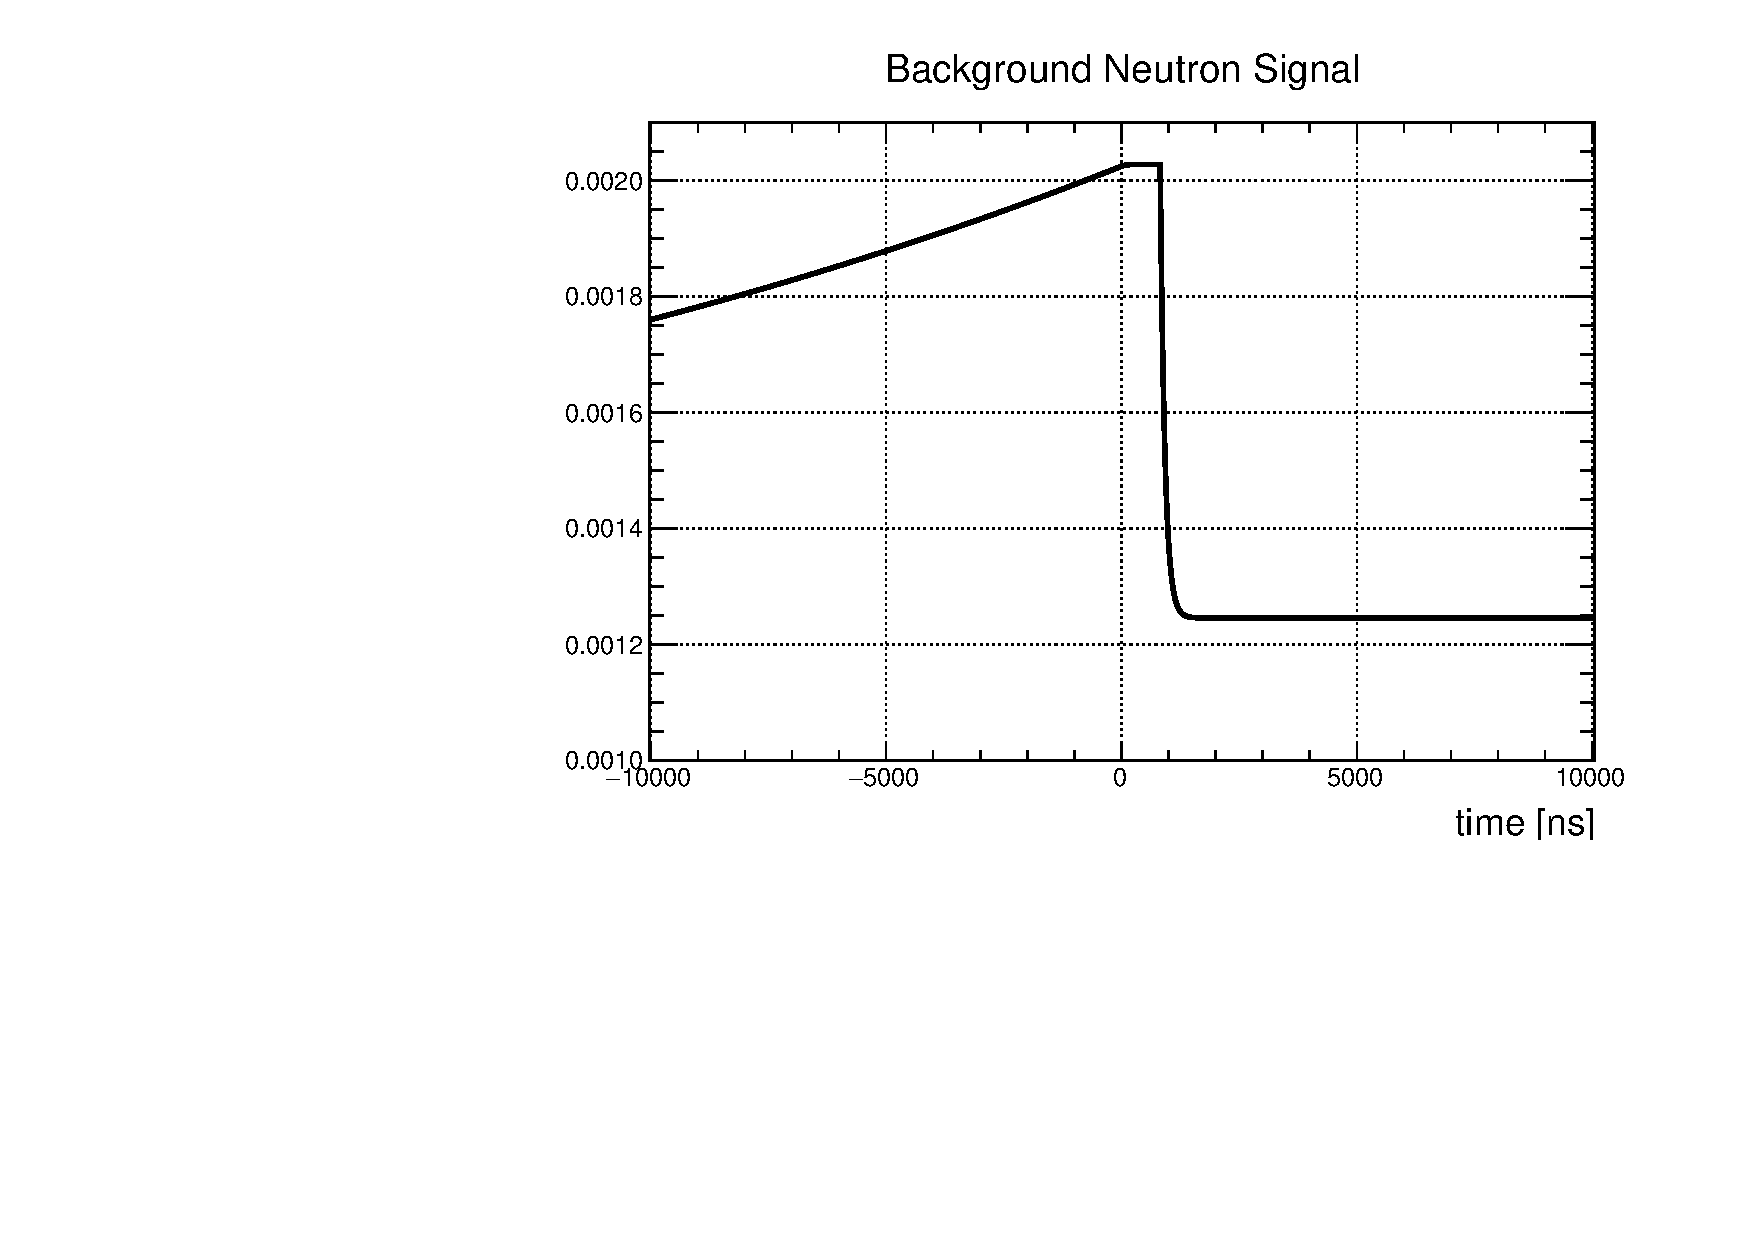
\includegraphics[width=\textwidth]{neutrons/figures/shape_neuBG.pdf}
  \caption{Neutron background signal for R2015 data.}
  \label{fig:shape_neubg}
\end{figure}

The beam background appears to be dominated by muon stops in the lead collimator at the front of the entrance detector stack.
Because these are essentially wall stops, they share many characteristics with the wall stop neutrons discussed previously. 
They have similar energy spectra, although it will differ somewhat due to stopping in lead rather than silver or tungsten.
They also consume the muon so there is no associated electron, although there are many uncorrelated beam electrons.

As the MuSun analysis requires a good muon entrance, these beam backgrounds only appear in the data if they are coincident with another muon.
Because a normal muon decay is by far the most probable result of any given stop, the neutron background is primarily composed of normal stops with an uncorrelated background neutron.
Using an electron veto can cut these events, but due to the electron detector solid angle coverage this only reduces the background by about two thirds.

Although the neutron background cannot be removed, we do have two different ways to isolate it.
First, we can study the neutron background using the muon clock just like any other background.
The clock simulates and event and triggers the kicker without any real muons present, so we can directly see the background effects.
While this is often helpful, the low neutron rates result in very low statistics in this case.

Alternatively, we can make a set of contradictory cuts to exclude as many other signals as possible.  
The TPC energy cut is effective at eliminating fusions, while a fiducial volume cut removes most wall stops and ensures no pulses are missed by the energy cut.
An electron requirement cuts most capture events as well, and the electron coincidence veto cuts photo-neutrons.
This leaves only normal decays with accidental neutrons, plus a small proportion of captures and photo-neutrons with accidental electrons.  
This method yields slightly more than four times the statistics of the clock data, at the cost of not completely eliminating the other signals.
It also has the benefit that it can be applied to periods when the clock was not active, including large portions of R2014.

\subsection{Photo-Neutrons}

Finally, the particles produced by muon capture or decay may undergo secondary reactions and produce additional neutrons.
Most commonly, high energy bremsstrahlung gamma rays may be absorbed in the walls and emit neutrons via photo-disintegration of the absorbing atom.
The resulting photo-neutrons will have a time dependence matching the electron signal, so essentially an exponential decay with the muon lifetime.
In fact, each photo-neutron should be coincident with the electron that originally emitted the gamma ray, but as usual electron cuts cannot conclusively identify events. 

The photo-neutrons are an important correction when studying the deuterium capture neutron signal.
Because the photo-neutrons are unaffected by the hyperfine states, any photo-neutrons in the capture spectra will result in underestimating the relative size of the fast component.
This in turn will produce skewed estimates of the quartet to doublet capture rate ratio.
A similar effect could also influence the kinetics calibration with the fusion neutrons, but the fusion signal is large enough that the effect should be small.

Photo-neutrons should also be produced by wall stops, either by bremsstrahlung photons again or by gammas emitted directly from the capture nucleus.
These photo-neutrons are not of much interest to us though, because they will have the same time dependence as the normal wall stop neutron signal and will simply result in a minor correction to the observed detection efficiency for these events.
Since the efficiencies are determined by fitting to the data in the first place, there is no real way to separate these signals.

The photo-neutron signal is quite small and therefore difficult to measure directly, so it is calibrated by fitting to positive muon data.
Unlike all of the other neutron signals described above which only apply to negative muons, the production of Photo-neutrons is independent of the muon charge.
Once the number of photo-neutrons has been determined from the positive muon data, it is assumed to scale with the number of muon entrances and kept fixed for fits to negative muon data.

Despite the connection between the photo-neutrons and gamma rays, it is difficult to determine the proportionality factor between them.  
One reason is that photo-neutrons are not related to gamma rays of the same energy, but rather gamma rays with high energies potentially exceeding the dynamic range of the neutron detectors.
In addition, the probability of a photo-disintegration event depends on the amount of material the gamma ray passes through, which in turn depends on the muon stop position and gamma emission direction.  

\section{Gamma Sources}

Recently there has been some interest in studying the gamma signals observed by the MuSun neutron detectors.
The gamma background has always been treated as a nuisance parameter for the neutron analysis, and significant effort went into trying to reduce them.
However, despite their name the neutron detectors see many more gammas than neutrons, so if any information can be extracted from them it would be quite useful.
We can identify four classes of gamma signal.

\subsection{Decay Electron Bremsstrahlung}

First, a large number of gammas are produced as bremsstrahlung radiation caused by muon decay electrons.  
As mentioned in the discussion of photo-neutrons, these gammas are coincident with an electron and follow the electron time distribution.
We could calibrate the bremsstrahlung photons based on the positive muon data as well, but in this case the signal is large and there are no similar signals to confuse it with so we can study it directly.
Comparing the signal between the positive and negative muons might help to verify that the photo-neutron calibration is working correctly though.

Bremsstrahlung gamma rays are produced by scattering in the detector structure and therefore depend on electron's path.
Somewhat counter-intuitively, having more material in the path produces a larger gamma signal since the electrons have a larger probability of scattering.
This produces significant changes in the signal depending on the specifics of the muon stop and electron emission direction.  
Most notably, there is often a difference of more than a factor of two between the neutron detectors above the target and those below.
This was a puzzle until we realized that the support structure below the TPC happens to be aligned with the lower neutron detectors, causing a large increase in observed scattering. 
Figure \ref{fig:epc_phi_z} shows the electron positions with and without neutrons selected, note how the shadows of the support beams align with the lower neutron detectors.
%todo - make a better figure

\begin{figure}[h]
  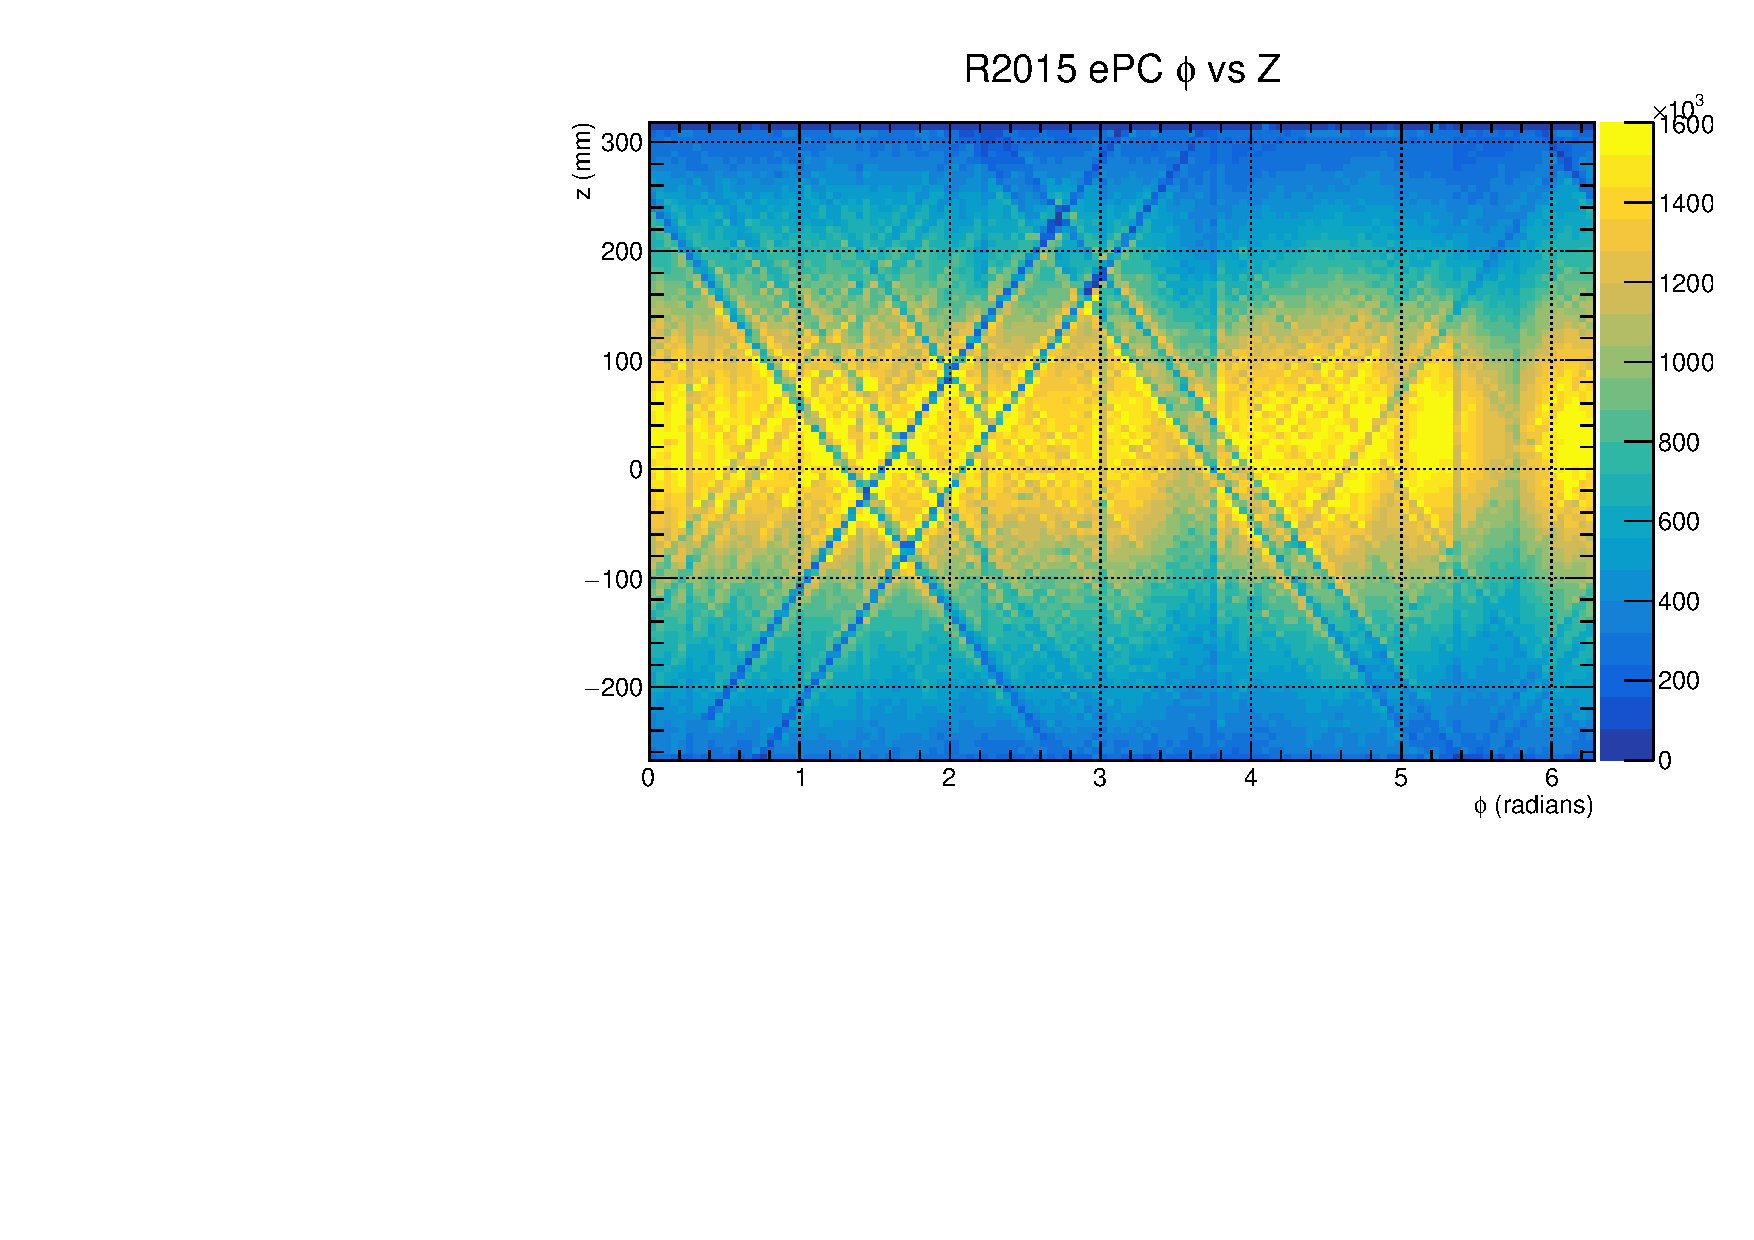
\includegraphics[width=0.49\textwidth]{neutrons/figures/ePC_phi_Z_All.pdf}
  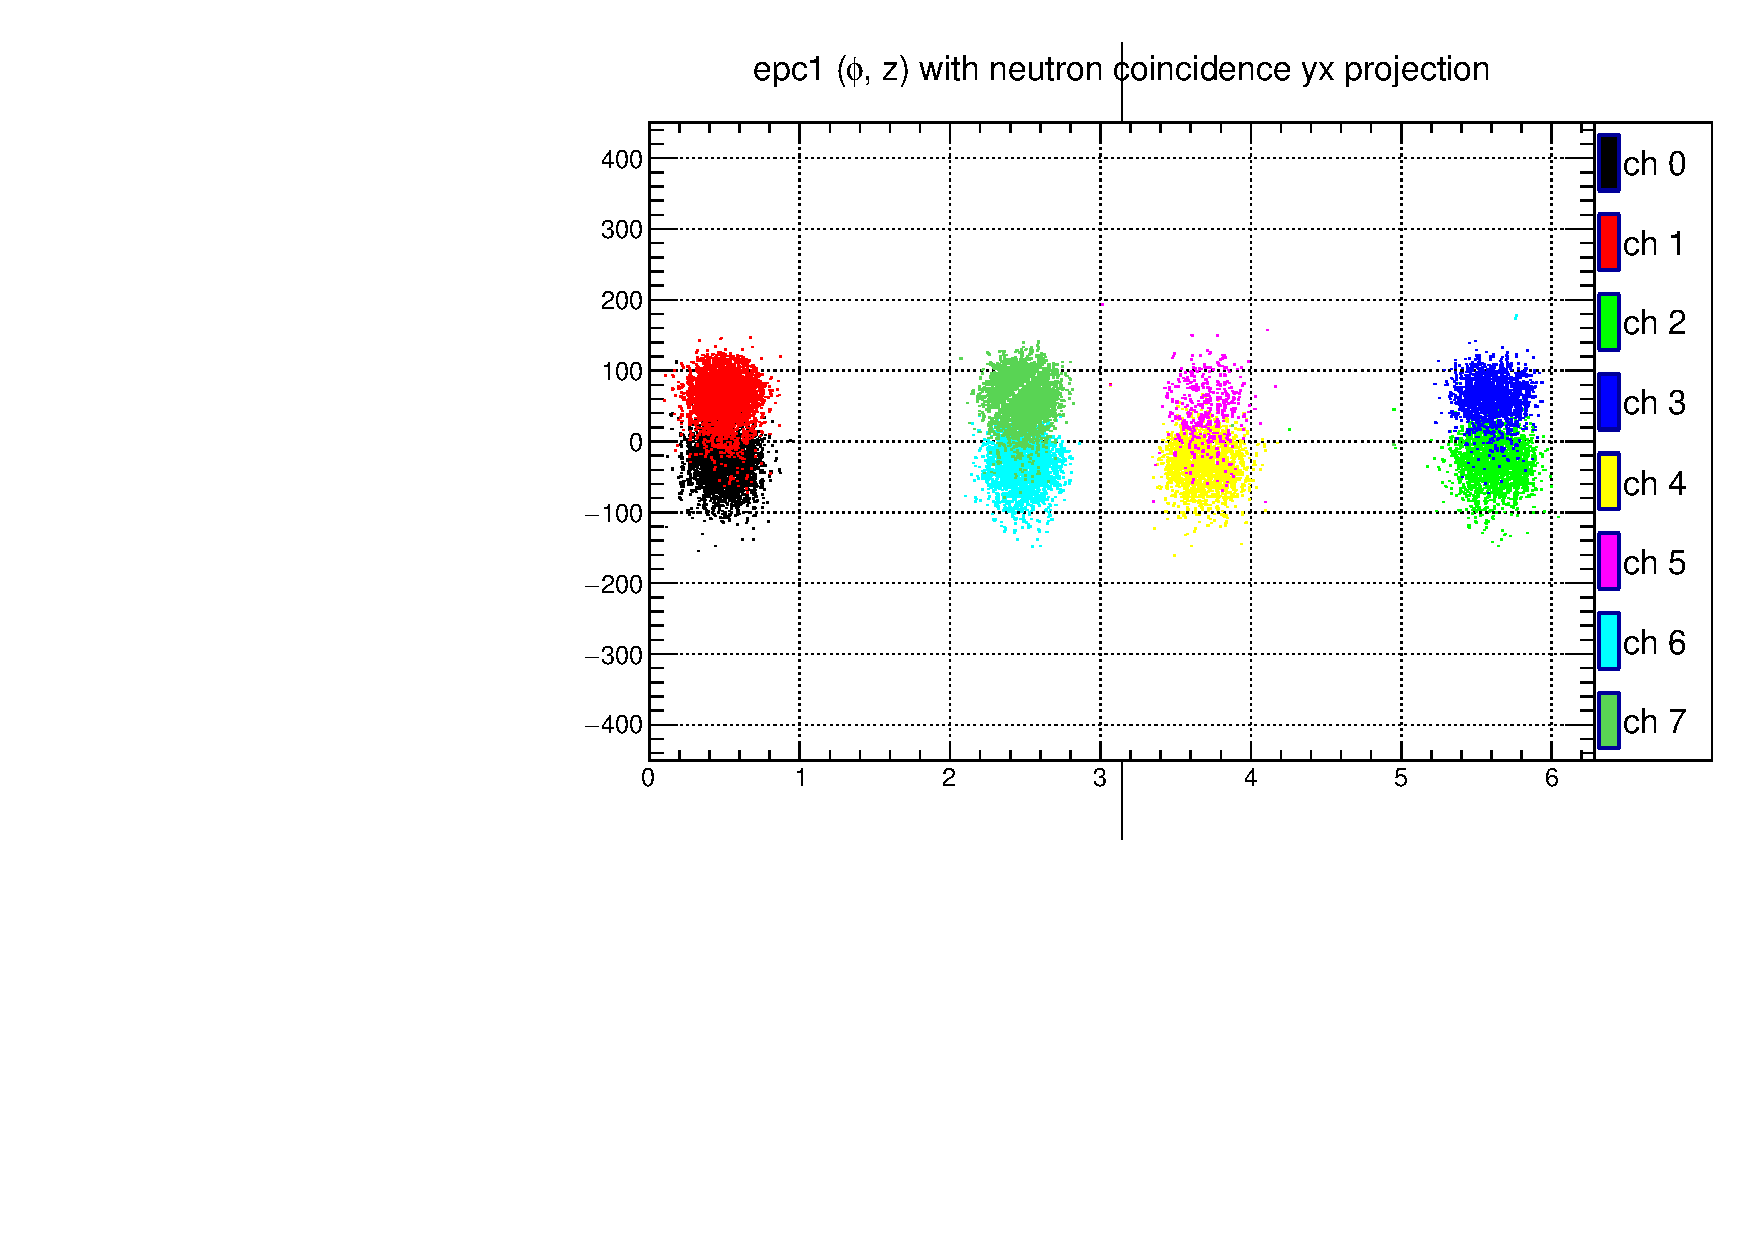
\includegraphics[width=0.49\textwidth]{neutrons/figures/ePC_phi_Z_Neu_Tagged.pdf}
  \caption{ePC $\phi$ vs Z for all R2015 data (left) and for events with a coincident neutron detector hit (right).}
  \label{fig:epc_phi_z}
\end{figure}

\subsection{Nuclear Capture}

Muon capture in deuterium splits the nucleus into a pair of unbound neutrons.
In higher-Z materials though, muon capture leaves behind a daughter nucleus which is often in an excited state.  
The nucleus will then quickly return to the ground state by emitting gamma rays.

Because these gamma rays are emitted immediately after muon capture, they follow the same exponential decay time distribution as the corresponding wall capture neutron signal.  
In principle these gamma rays should form distinct transition lines, but the complicated structure of high-Z nuclei produces a large number of closely spaced transitions.
These lines are then smeared together by the MuSun neutron detector response, making any detailed study of the spectrum hopeless.
The nuclear capture gammas therefore seem to only be useful as an additional indicator of wall stops.

\subsection{Atomic Capture}

The most interesting feature of the gamma ray signals is the ability to observe gammas emitted during atomic capture. 
When muons are captured by an atom, they initially start at very high energy levels of n=20 or more.  %todo citation
The muon then rapidly cascades down to the atomic ground state, emitting gammas with well-defined transition energies in the process.
This cascade process takes less than ten nanoseconds, producing a large gamma peak coincident with the muon entrance.
In principle, the pulse should have a complicated structure since it originates from several atomic transitions occurring in turn with delays in between.
In practice these considerations are unimportant as the pulse shape seems to be entirely dominated by detector response effects.

Energy spectra for these prompt gammas from various target materials were observed in the 2016 calibration run, and are shown in figure \ref{fig:atomic_lines}. 
The transition lines in deuterium have too little energy to be observable by the MuSun neutron detectors, but the $2 \rightarrow 1$ and $3 \rightarrow 2$ transitions are clearly visible for high-Z materials.
The transition energies give us an additional way to identify the stop materials which is more accurate than estimating the capture rate.
If the stop material distribution is well known, that can also be used to fix the capture rate used in the rest of the analysis.

\begin{figure}[h]
  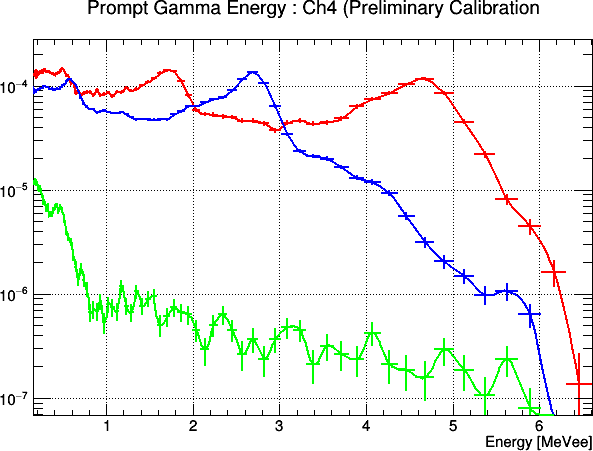
\includegraphics[width=\textwidth]{neutrons/figures/PromptGamma_EnergiesCh4.png}
  \caption{Atomic capture gamma energy spectra from R2016 calibration data.}
  \label{fig:atomic_lines}
\end{figure}

The atomic capture gamma (ACG) pulse is a very distinctive signature of high-Z wall stops. 
Because the pulse is so short it has a high signal to background ratio even with very few events and can be used to detect wall stops with comparable sensitivity to the capture neutrons themselves.
However, the peak lies directly on the steep rising edge of the other exponential distributions.
This makes the peak correlated to the relative time offsets of the signals, which should be close to zero but are not entirely certain.
Thus, although the pulse gives a very precise measure of wall stops it can have a small systematic bias which is hard to calibrate.

The Macor signal is much smaller and lacks the clean high-energy peaks of the high-Z materials, but still emits a noticable pulse of lower energy gammas.
Because the muon capture rate in macor is much lower than in the other TPC materials, stops in macor are very hard to detect by looking for capture neutrons.
In this case, the ACG signal may prove much more useful than the neutrons for identifying such stops.

\subsection{Beam Background}

Finally, there is a large beam background gamma ray signal.
This signal is mostly due to bremsstrahlung radiation from particles in the beam.
The beam gamma background increases when the kicker is fired, since it follows the electron background which also increases.

To study the gamma background, we may again use either the muon clock data or the conflicting cuts approach.
The high number of bremsstrahlung gammas makes the cut method less attractive, and there are enough gamma events that the clock gives decent statistics.
Calibrating with the clock data, we extract the background shape seen in figure \ref{fig:shape_gammabg}.

\begin{figure}[h]
  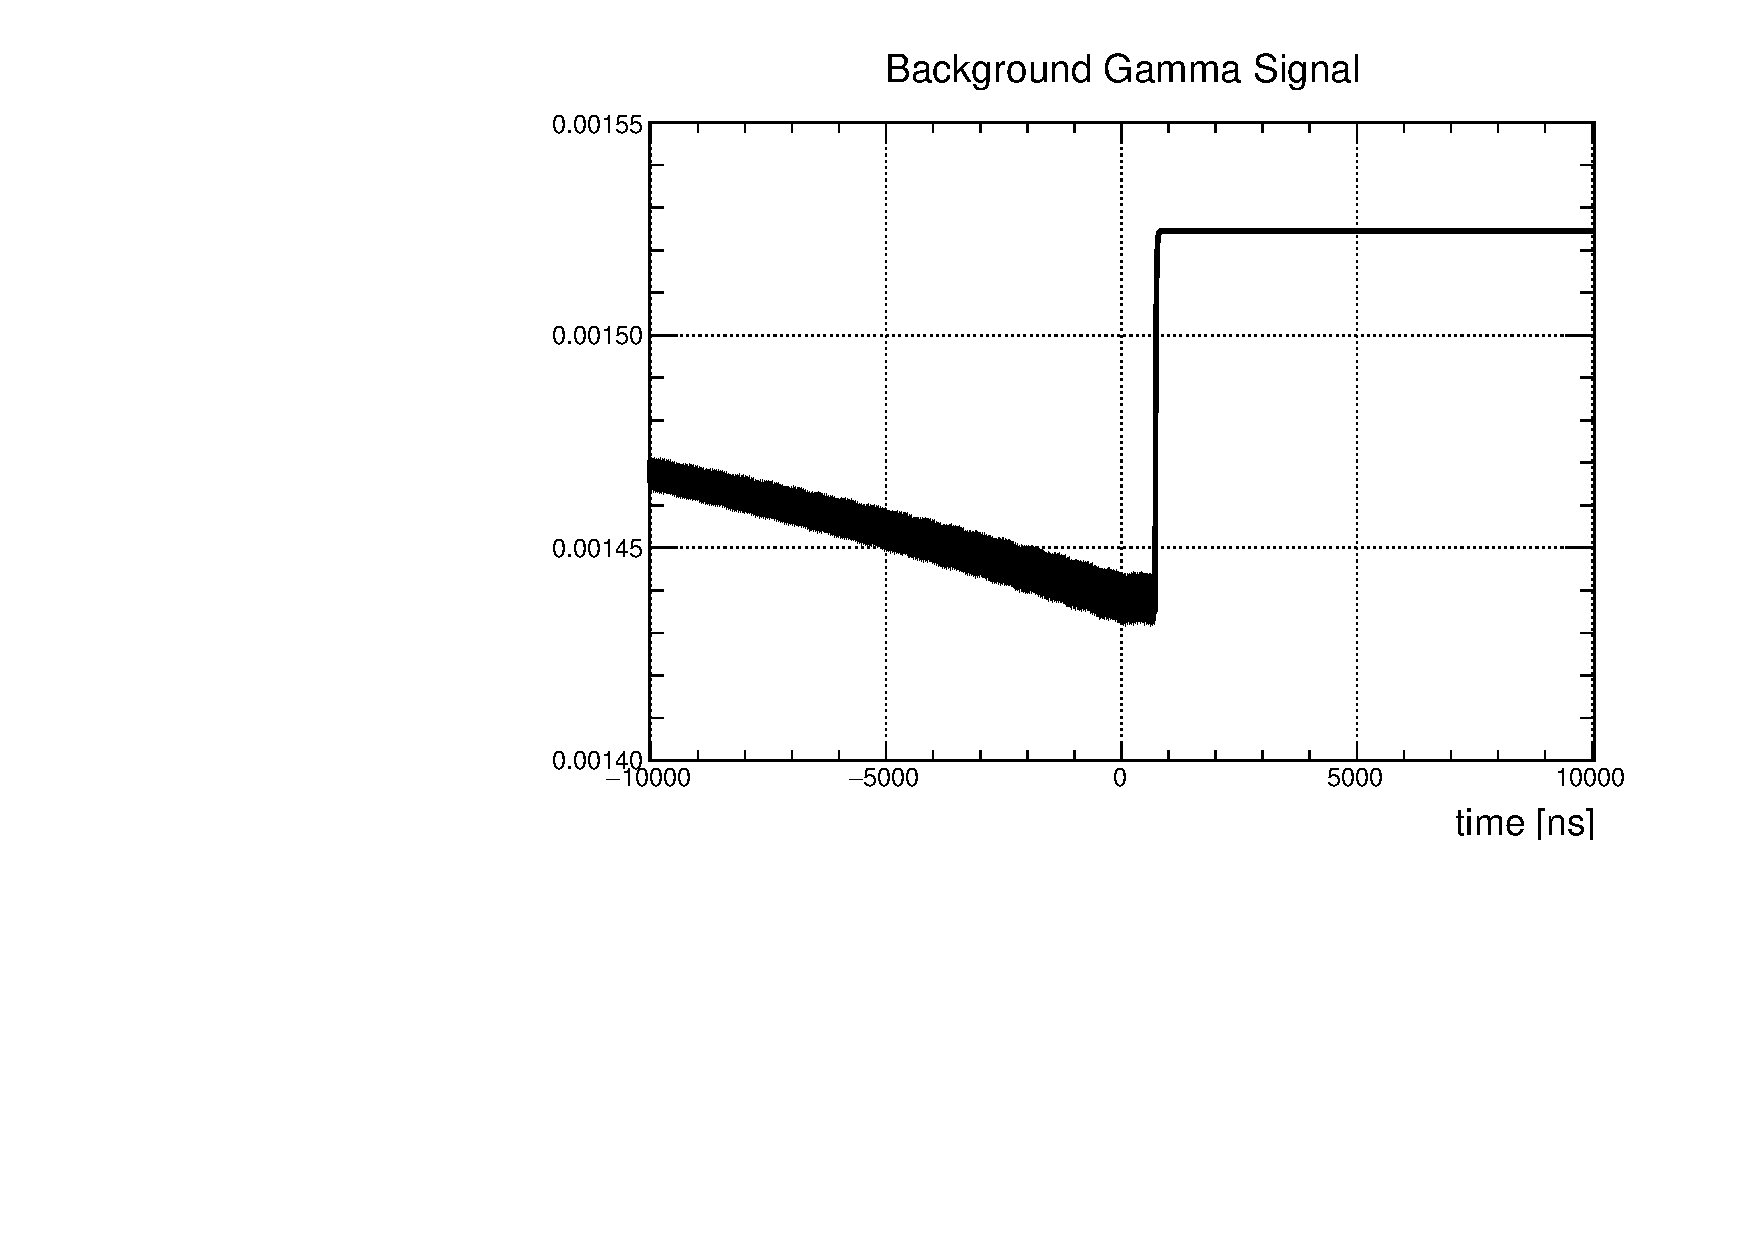
\includegraphics[width=\textwidth]{neutrons/figures/shape_gammaBG.pdf}
  \caption{Gamma background signal for R2015 data.}
  \label{fig:shape_gammabg}
\end{figure}

Unlike the neutron background, the gamma background also includes the accelerator RF oscillations.  
The oscillation does not interfere with the other signals, so it can be fit directly to the real data using a specialized oscillation histogram.  
This histogram saves the time modulo the RF frequency for gammas occurring either before the muon entrance or more than 10 $\mu s$ after the entrance, avoiding the region with large signals and complicated time dependence.
The kicked oscillations are fit directly to the late time signal.
The un-kicked oscillations parameters are determined by fitting the early time signal and subtracting the expected amplitude from the kicked oscillations.
I assume the oscillation phase is the same for the kicked and un-kicked beam configurations.
An example fit is shown in figure \ref{fig:rf_calib}. 
An identical histogram is generated for the neutron background, but no oscillations are apparent so the oscillation amplitude is fixed to zero.

\begin{figure}[h]
  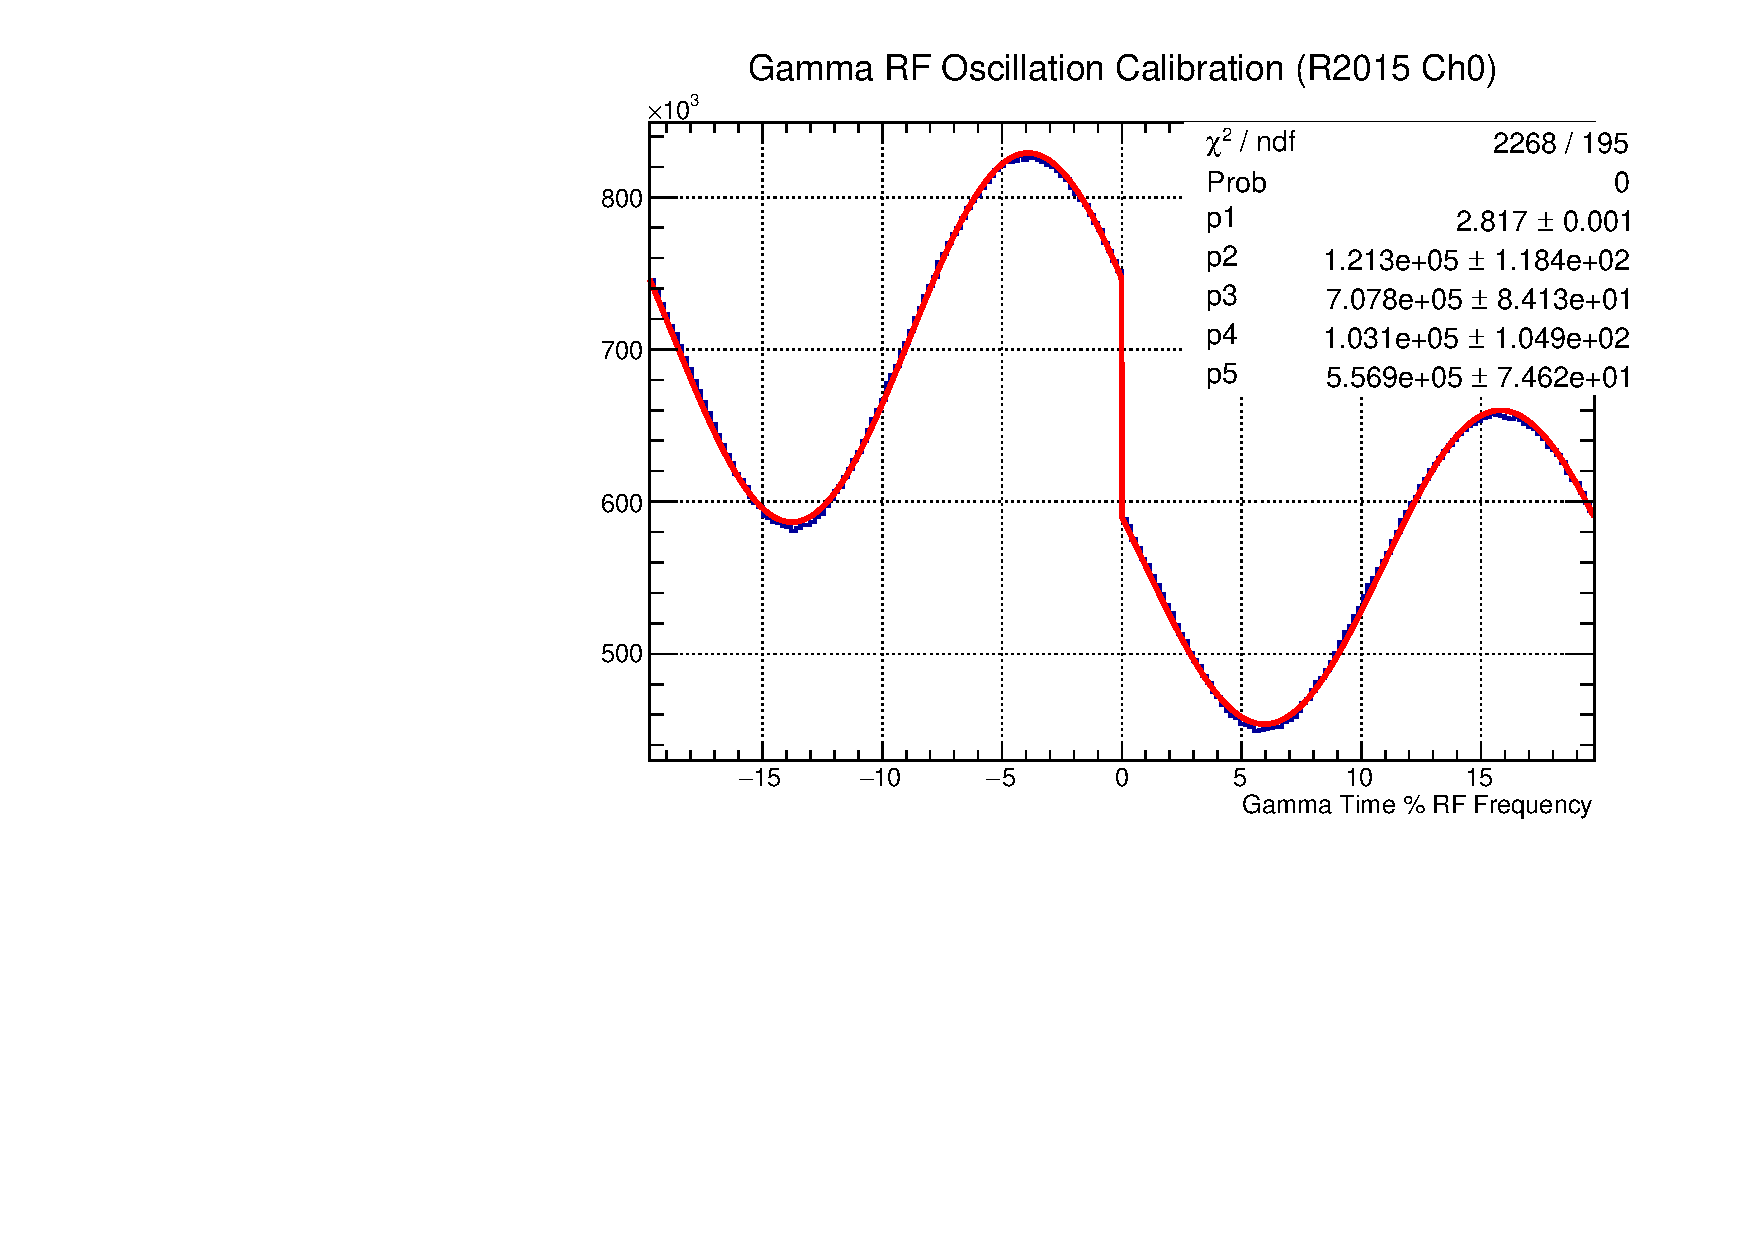
\includegraphics[width=\textwidth]{neutrons/figures/RF_oscillation_calib.pdf}
  \caption{RF oscillation histogram with fit to sine waves with constant backgrounds.  The $\chi^2$ value is poor because the slopes of the background are not modeled, but the oscillation parameters should be reliable.}
  \label{fig:rf_calib}
\end{figure}

\begin{table}[h]
  \begin{center}
    \caption{Neutron detector signal summary}
    \label{tab:signal_summary}
    \begin{tabular}{ | l | l | l | l | l | l | }
      \hline
      Particle  & Signal          & Electron  & Energy  & Source      & Special Properties        \\
      \hline
      Neutron   & D Capture       & none      & smooth  & D stops     & two simultaneous neutrons \\
                & $^3$He Fusion   & delayed   & peaked  & D stops     & additional TPC energy     \\
                & High-Z Capture  & none      & smooth  & wall stops  & \\
                & Background      & present   & smooth  & beam        & \\
                & Photo-Neutrons  & prompt    & smooth  & scattering  & \\
      \hline
      Gamma     & Electron Brem.  & prompt    & smooth  & scattering  & \\
                & Nuclear Capture & none      & smooth  & wall stops  & \\
                & Atomic Capture  & none      & peaked  & wall stops  & coincident with muon      \\
                & Background      & present   & smooth  & beam        & \\
      \hline
    \end{tabular}
  \end{center}
\end{table}

\section{PSD Calibration}

As mentioned in chapter \ref{ch:software}, pulses caused by neutrons may be identified by their long tails following the initial peak.
A pulse shape discrimination (PSD) cut is defined based on the fraction of the pulse area contained in the pulse tail.
The pulse shapes change slightly with pulse energy so the PSD cut is also energy dependent, and plots of pulse tail fraction vs total area are referred to as PSD plots.

Now that the possible neutron and gamma signals are well understood, we can use that information to refine the PSD cuts and estimate their error rates.
By selecting fusion events with a TPC energy cut or selecting stops near the walls to maximize high-Z captures, we may produce a distribution with a much higher proportion of neutrons than usual.  
Similarly, a distribution with predominantly gamma rays may be created by selecting events with a coincident muon entrance or electron.
Figure \ref{fig:psd_selection} shows PSD plots with these cuts applied:

\begin{figure}[h]
  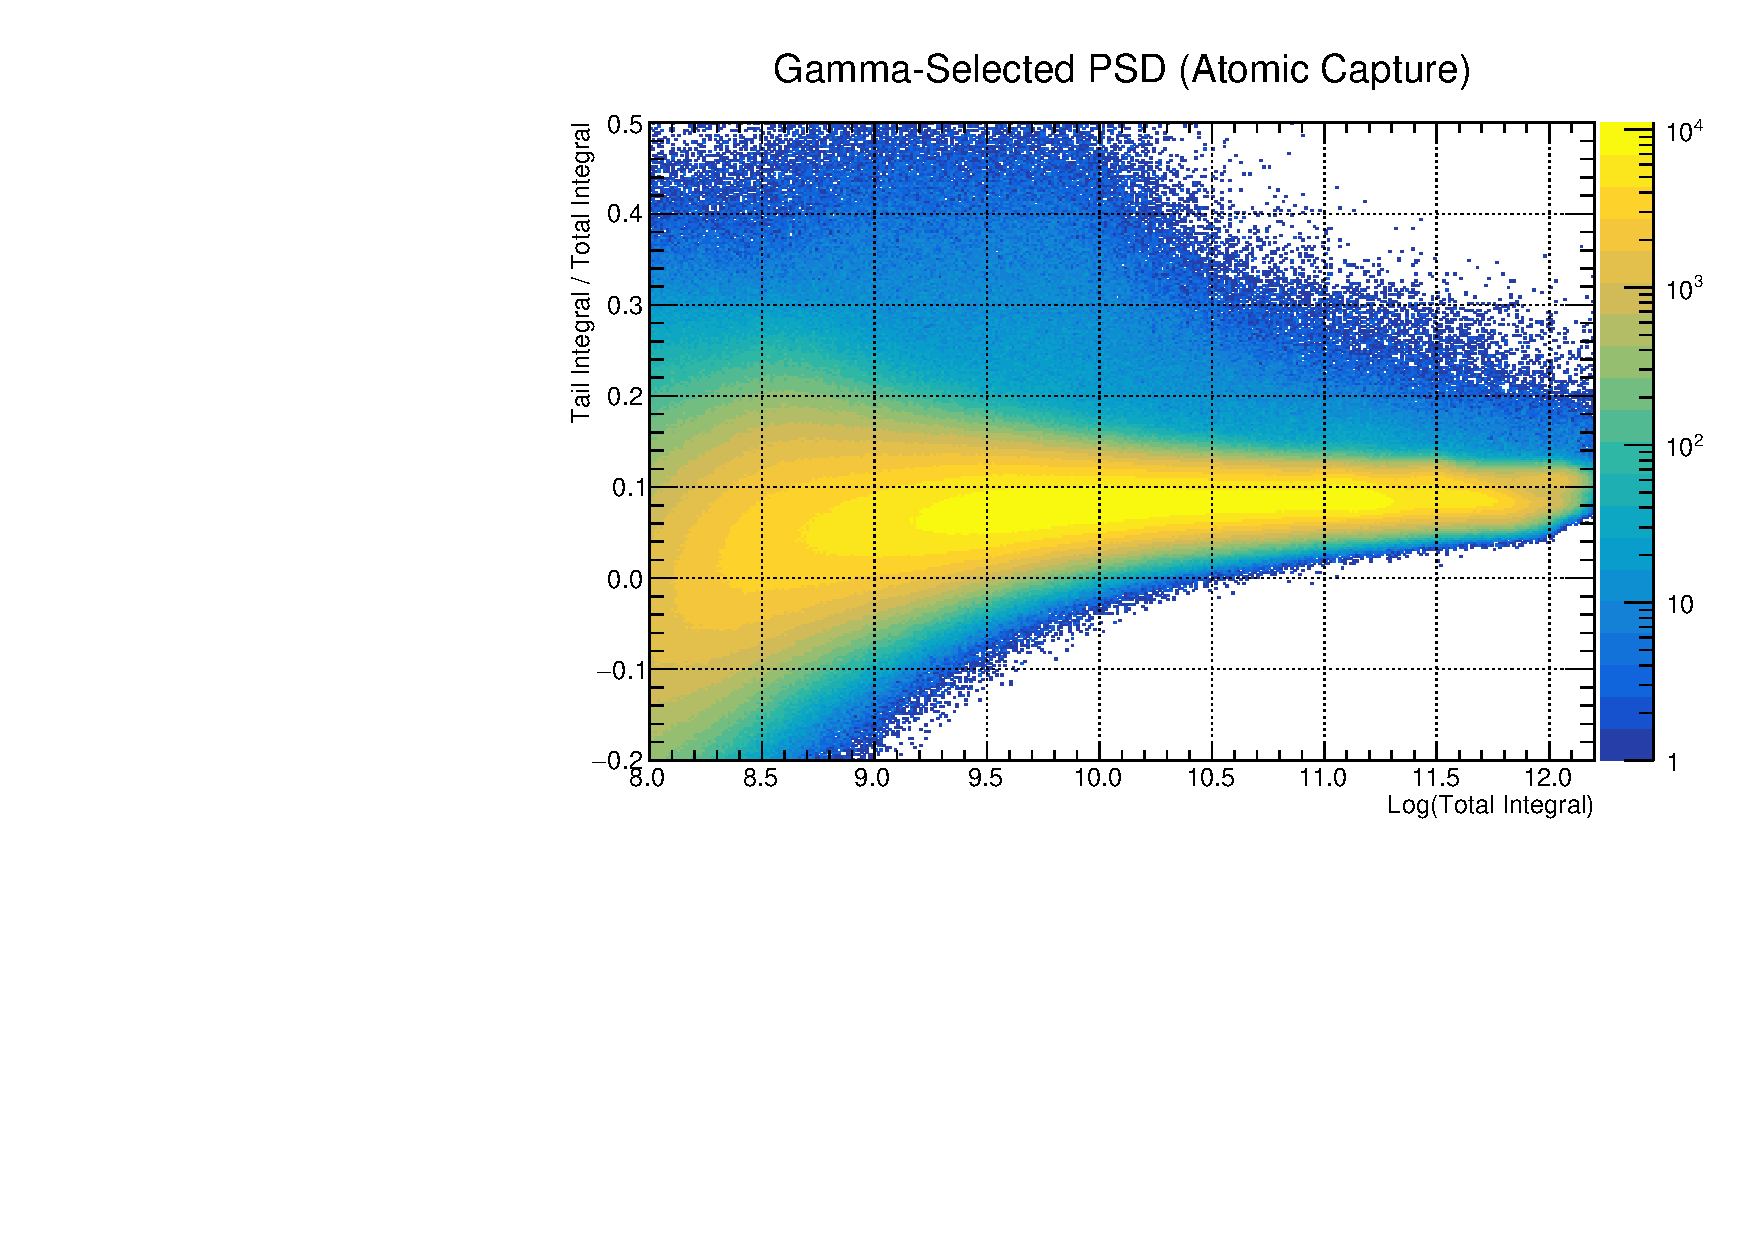
\includegraphics[width=0.49\textwidth]{neutrons/figures/PSD_gammma_atomic.pdf}
  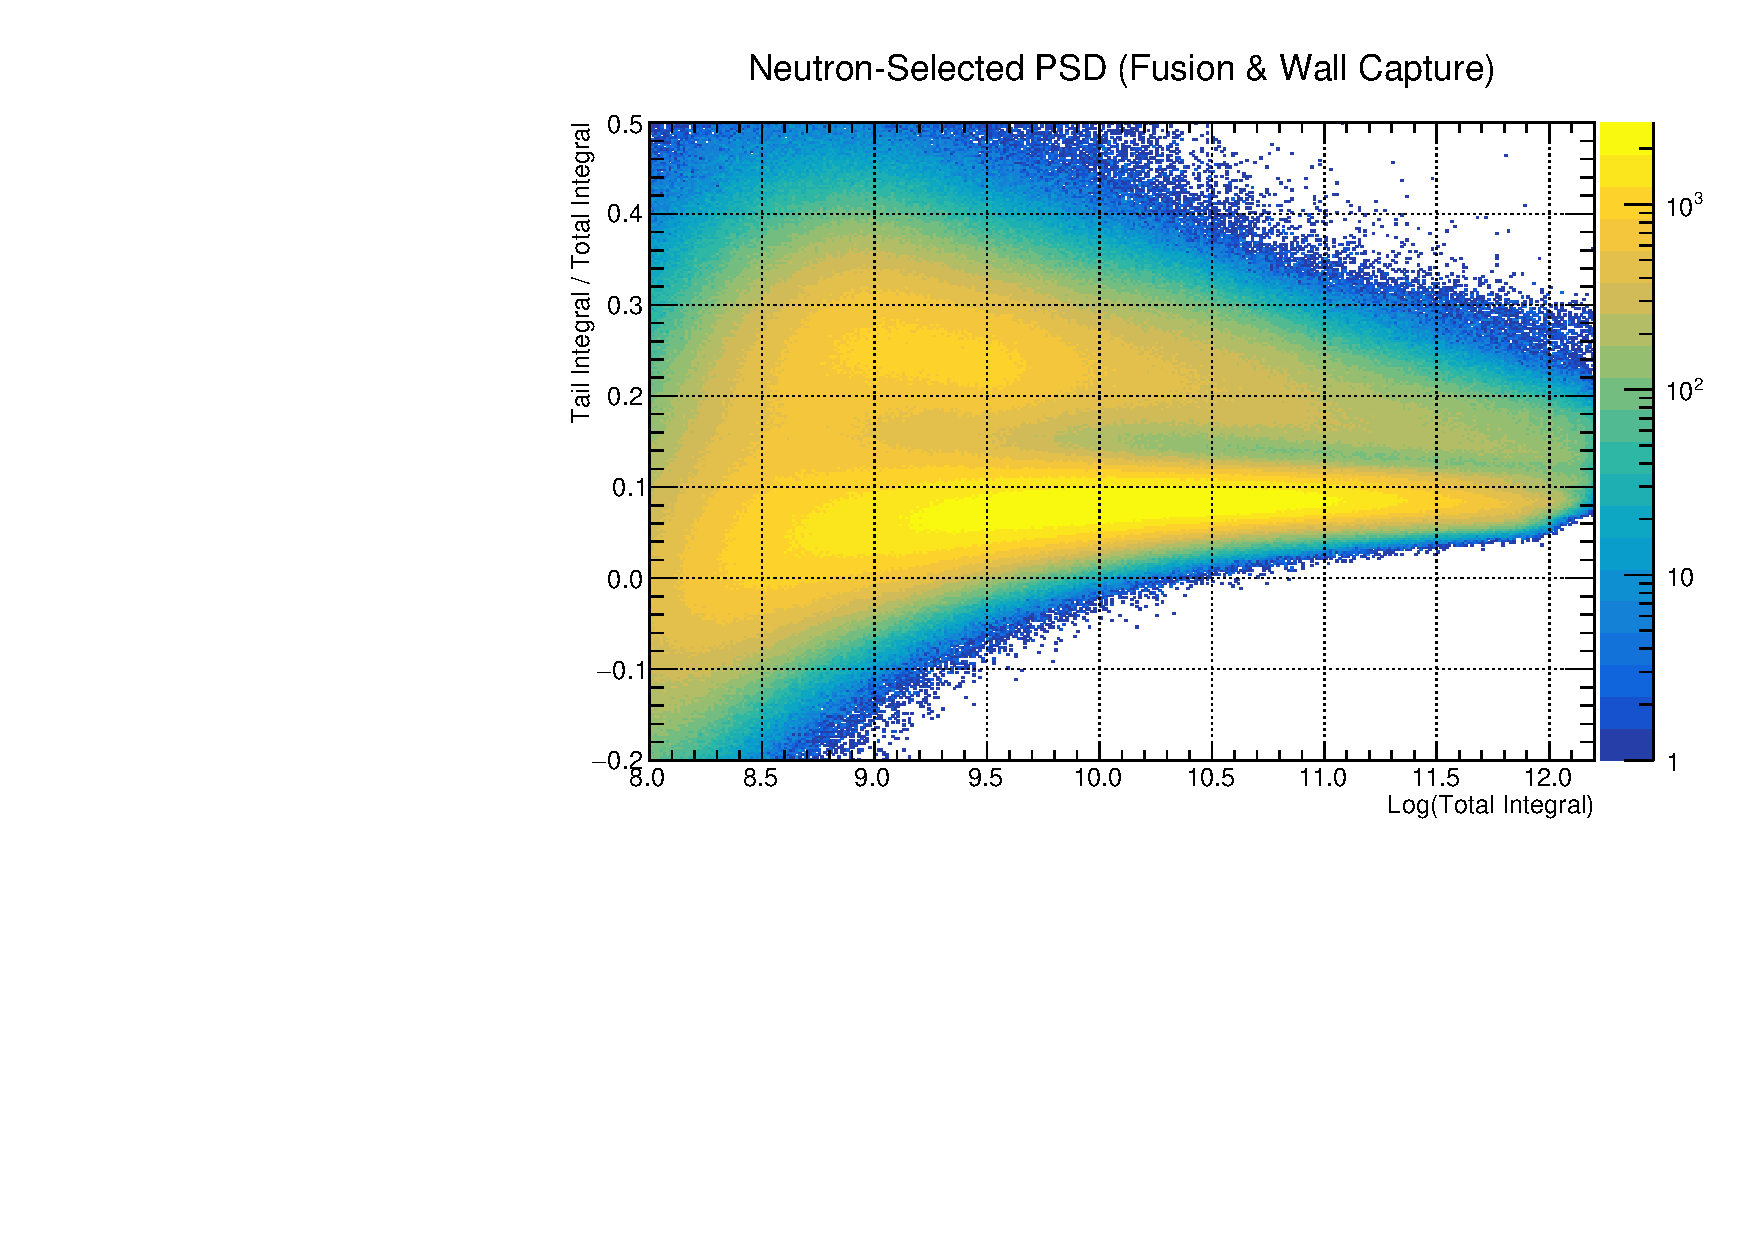
\includegraphics[width=0.49\textwidth]{neutrons/figures/PSD_neu_fusion_wall.pdf}
  \caption{PSD plots with either atomic capture gammas (left) or wall stop and fusion neutrons selected (right)}
  \label{fig:psd_selection}
\end{figure}

For each energy slice, we attempt to separate these two distributions into pure neutron and gamma distributions.  
If $F_1$ and $F_2$ refer to the gamma and neutron selected events respectively, we can write them in terms of the true distributions $F_{\gamma}$ and $F_n$:
\begin{align}
F_1 & = N_{1\gamma} F_{\gamma} + N_{1n} F_n \\
F_2 & = N_{2\gamma} F_{\gamma} + N_{2n} F_n 
\end{align}
where the N's are the numbers of each kind of event in either set.
If we knew these values then extracting the true distributions would be a simple matter of scaling and subtracting the two histograms:
\begin{align}
F_{\gamma} & = (F_1 N_{2n} - F_2 N_{1n}) / (N_{1\gamma} N_{2n} - N_{2\gamma} N_{1n}) \\
F_n & = (F_2 N_{1\gamma} - F_1 N_{2\gamma}) / (N_{1\gamma} N_{2n} - N_{2\gamma} N_{1n})
\end{align}

In practice, the proportion of neutrons and gammas in each set is unknown.  
Rough estimates may be obtained by fitting the neutron and gamma bands to a pair of gaussians, but overlap between the bands and any differences in their true shapes will produce errors with this method.
More accurate values may be determined using the shape fitting method discussed in the next section.

Extraction of the true distributions is also somewhat problematic due to the statistical fluctuations of the data.  
The gamma-selected distribution is already quite pure, so subtracting a small proportion of neutrons has little effect.
Neutrons cannot be selected with the same accuracy however, and the best neutron-selected distribution still has a majority of gamma events.
Scaling and subtracting the gamma distribution therefore leaves large fluctuations in the place of the original gamma band.
To mitigate this issue, the resulting distributions are smoothed before being analyzed further.

\begin{figure}[h]
  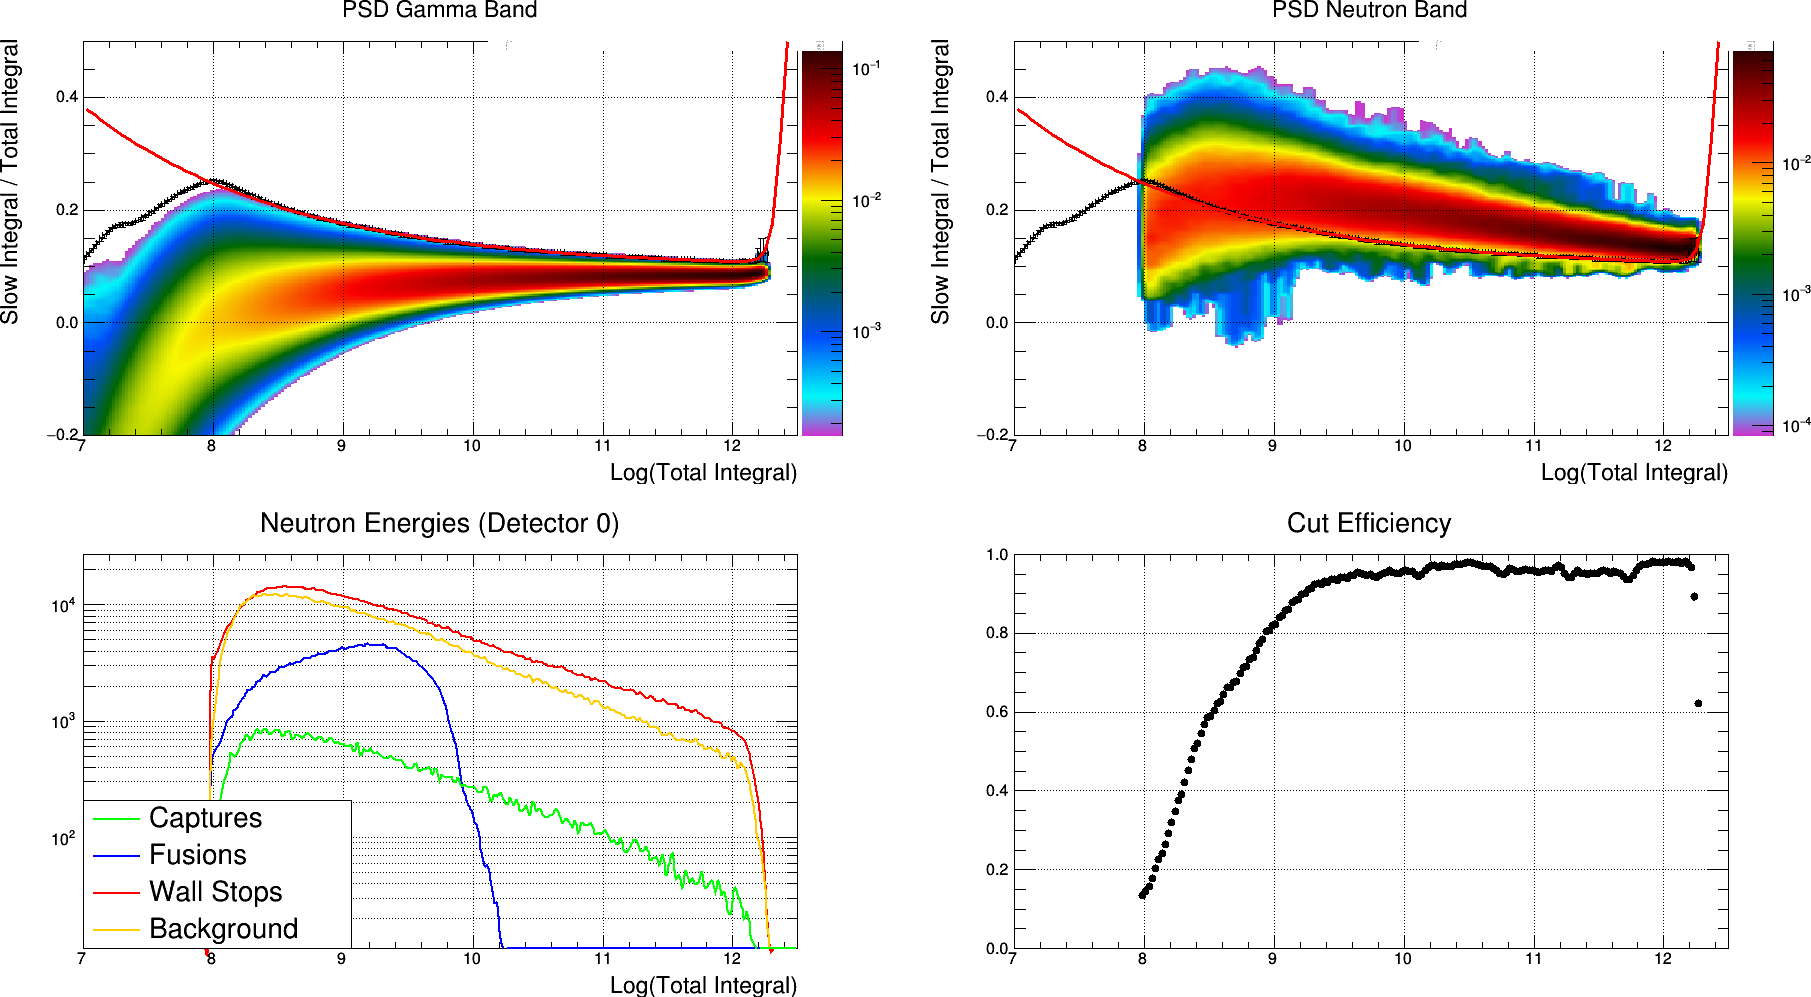
\includegraphics[width=\textwidth]{neutrons/figures/PSD_fit.png}
  \caption{PSD plots of the estimated true gamma (left) and neutron bands (right)}
  \label{fig:psd_fit}
\end{figure}

Finally, a PSD cut is defined based on the estimated pure distributions.
Because the gamma signal is so large, our PSD cuts have been designed to suppress the gammas by various proportions.
Figure \ref{fig:psd_fit} shows pure distributions extracted from the data in figure \ref{fig:psd_selection} along with a PSD cut set to reduce the gamma signal by a factor of $10^{4}$.
The neutron band is not used for setting the PSD cut, but is used to determine the cut efficiency.

\section{Time Distribution Fitting}

With the exception of fusion neutrons which may be identified relatively easily, the most distinctive characteristic of the other signals is their time dependence.  
The time distributions of the signals overlap, so it is generally not possible to identify individual events with time cuts.  
However, by fitting the time distribution we can determine the number of events of each type.
A fitting procedure designed to determine these signal components has been developed using RooFit.

\subsection{Signal Models}

RooFit models are built using probability density functions (PDFs).  
RooFit provides some generic PDF classes by default, but we have created a modified base class with two important features.
First, the PDFs support a software blinding scheme which scales the time variable before it is passed to the actual fit function.
This scaling mimics our hardware blinding of the master clock rate, and is equivalent to blinding all relevant rates by a given fraction.
Second, we have implemented an optional binned fitting mode where the integral of the fit function is used, as opposed to the default RooFit behavior of simply fitting the function at the bin centers.  
This mode respects variable binning schemes, which allows the use of narrow time bins to capture the initial gamma pulse and sharp increase in signal after the muon entrance.  
Currently, we use 1 ns binning within $\pm$20 ns of the entrance, 10 ns binning within the first 2 $\mu$s, and 100 ns binning otherwise.

The expected time distributions from each signal source are then defined as custom PDF classes derived from our modified base class.
We need a total of four different PDFs to describe all the signals:
\begin{itemize}
  \item Photo-neutrons, bremsstrahlung, and neutrons and gammas from high-Z captures all have simple exponential distributions. 
  \item Neutrons from deuterium capture and $^3$He fusion follow a double-exponential distribution.
  \item The backgrounds are well-described by the background model described in \ref{ch:beam_bg}.
  \item The atomic capture gamma peak requires its own PDF.
\end{itemize}

A first approximation to the signal shapes gives us discontinuous functions where the signal suddenly increases after the muon stop.  
This is clearly unphysical, and we would like a continuous function to fit to the data.
There is some time dependence to the muon stop, but the dominant effects in the signal are the finite detector resolution and time of flight differences smearing the signal.
We model this smearing using a convolution with a gaussian kernel, transforming the exponential decays into shapes known as exponentially modified gaussians.
The resulting PDF has two free parameters: the width of the kernel and the start time of the signal.  

The ACG pulse is wider than expected and does not fit well to a gaussian.
This peak is currently modeled as a square pulse convolved with a gaussian smearing kernel, which seems to approximate the observed signal.
The resulting PDF therefore has three parameters: the time of the peak and the widths of the square pulse and kernel.
The width of the square pulse is most likely related to issues with the neutron pulse interpolation, and may be eliminated with improvements to the algorithm. 

The background shapes discussed in chapter \ref{ch:beam_bg} are already continuous functions so it is not necessary to apply an additional convolution.
Any smearing due to timing uncertainty will only have a noticeable effect on the shape of the kicker step, and this can already be accounted for by the existing adjustable parameters of the model.

\subsection{Free Parameter Reduction}

At this point the fit model has quite a large number of free parameters.  
For each of the eight detectors we have seven signals each with amplitude, time, and width parameters, as well as all the parameters in the background model.
There are also all of the muon kinetics parameters which we may wish to leave floating for some analyses.  
With so many parameters the fits become unreliable and unlikely to converge, so it is important to reduce the parameters as much as possible.

\subsubsection{Simultaneous Fitting}

One important way to reduce the free parameters is to fit all of the neutron data simultaneously. 
Using the RooFit framework makes this simple, and given fit models for individual neutron and gamma channels we can easily create a combined fit to the signals from all eight detectors together.
A resulting combined fit is shown in figure \ref{fig:multi_fit}, with the colors showing the effects of each signal source being added in turn.

\begin{figure}[h]
  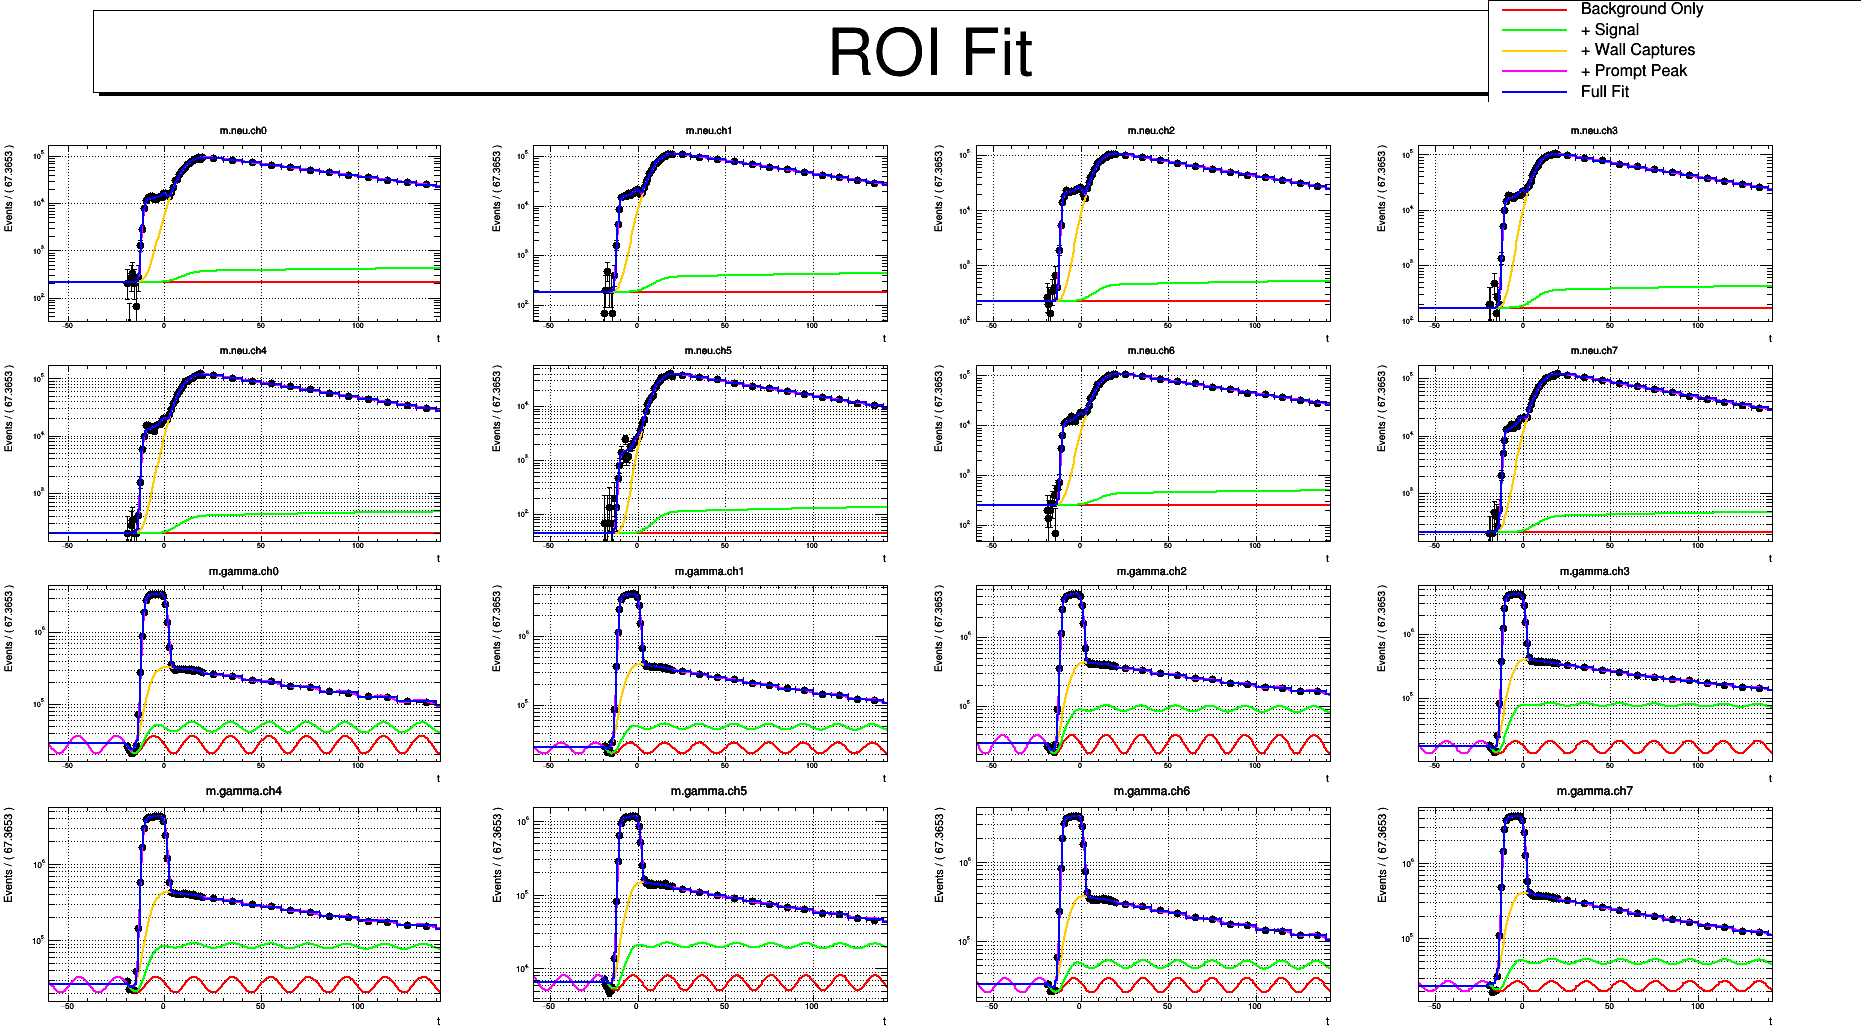
\includegraphics[width=\textwidth]{neutrons/figures/multifit_ROI_Zoom.png}
  \caption{Combined fit to all detector channels for R2015 stops in the ROI.}
  \label{fig:multi_fit}
\end{figure}

By doing this simultaneous fit, we can force the different channels to share a single variable when appropriate.  
For example, the detectors are all observing the same physics, so physical properties such as decay rates and muon kinetics parameters should not depend on the specific detector being studied.
Compared to letting these parameters float separately fitting each of the sixteen histograms, the combined fit yields a much better determination of the parameters while simultaneously ensuring that the results are consistent across the detectors.

Another benefit of the simultaneous fit is that some signals may be defined relative to others.  
The best instance of this is the photo-neutron signal, which is difficult to directly measure as discussed above.  
Instead, the photo-neutron signal is constrained to be proportional to the gamma ray signal in the same detector.  
Similarly, contamination of the signals due to the imperfection of the PSD cut may be accounted for by adding a component in the neutron fit proportional to the gamma signal and vice versa.
This is most apparent in the ACG peak, which manifests as a shoulder on the rising edge of the neutron signals, but may also produce a significant fusion component in the gamma histograms.

\subsubsection{Timing}

In general we would expect the the observed signals to have the same shape in all detectors.  
However, the detectors may have individual time offsets and possibly somewhat different time resolutions as well.
The observed offsets and resolutions are partially intrinsic to the detectors but also have a component caused by the time of flight of particles in the detector.

For gamma rays precise timing is important to isolate the ACG peak as much as possible, and we can model the time of flight fairly accurately.
The time of flight has two components: first the muon must travel from the entrance detectors to the stop location, and then the gamma ray travels from the stop to the detector.
Because the upstream beam slits only accept a narrow momentum slice, all incoming muons have nearly the same speed of $v_{\mu} \approx 1/3 c$. 
The time of flight is then given by the equation
\begin{equation}
\Delta t = v_{\mu} \lvert \vec{r}_{stop}-\vec{r}_{ent} \rvert + c \lvert \vec{r}_{stop}-\vec{r}_{det} \rvert
\end{equation}
where $\vec{r}_{stop}$, $\vec{r}_{ent}$, and $\vec{r}_{det}$ denote the positions of the muon stop, entrance window, and neutron detector respectively.
Apart from the time of flight, the time resolution seems to be similar for all gamma ray signals so they are combined into a single parameter.

Correcting for the neutron flight time is a more difficult proposition, because the neutrons are produced with a range of energies and therefore a range of velocities.  
Furthermore, since neutrons scattering in the detector only deposit a fraction of their total energy we cannot easily estimate the neutron speed from the observed energy.
Fortunately, without the ACG peak it is much less critical to get precise time information for the neutrons.
The time of flight for the neutrons is therefore not modeled, and appears as an additional broadening visible in the neutron signals in figure \ref{fig:multi_fit}.

The width and time offsets of the various neutron signals should be directly related to their energy spectra, but apart from the fusion neutrons the other signals have similar distributions.  
For our purposes using a single width parameter for all of these signals is sufficient.
%todo - take a look at fusion neutron width.
The seven DEMON detectors also appear roughly similar, but detector 5 is one of the old BICRON detectors and does not match the others due to its different energy sensitivity.

\subsubsection{Solid Angle Correction}

Another tempting way to eliminate redundant fit parameters is to use a single parameter to describe the strength of each signal component across detectors.
After all, the detectors are all observing the same reactions and should produce signals proportional to the reaction rate multiplied by the detector efficiency.
However, this becomes more complicated when we consider how the detection efficiency varies with the muon stop position.
This depends on the source of the signal, which may be divided into three classes:

\begin{description}
\item[Beam Backgrounds] are the simplest signals to account for.  
These are uncorrelated with the observed muon stop by definition, so the muon properties are irrelevant and the backgrounds scale directly with the number of muon entrances.
%todo - check effect of electron cuts
The individual detector efficiencies must still be calibrated, but subsequent fits may use a single background strength parameter or even fix the backgrounds relative to the number of muon entrances leaving zero free parameters.

\item[Direct Signals] emitted by interactions of the muon radiate outwards from the muon stop location, so the observed signal strength depends on the proximity of the stop to the detector.
These signals include capture and fusion neutrons as well as atomic and nuclear capture gamma rays.
A correction is applied to these signals by calculating the solid angle coverage of each detector integrated over stop position.
With the solid angle correction applied, these signals also require only a single amplitude parameter each.

Currently events are treated as if they stop uniformly across the TPC pad area, and minor improvements may be possible with more complicated interpolation.
Another problem is that signals associated with interactions in the bulk deuterium and signals from wall stops should clearly use different stop distributions for the solid angle correction.  
This issue becomes less important with a smaller region selected, so it should be possible to iteratively map out the wall stop distribution and then apply the resulting distribution for future solid angle corrections.
%todo - make better interpolation and figure out errors.

\item[Scattering] events such as bremsstrahlung and photo-neutron signals originate from interactions in the TPC walls rather than directly from the muon.
The signal strength depends therefore depends on the geometry of the detectors and support structure and does not follow a simple pattern like the other signals.
It may be possible to use Monte Carlo simulation data to estimate the detection efficiency as a function of stop position, but it is uncertain how applicable this would be to real data.  
For now, these signals require a separate amplitude parameter for each detector.
\end{description}

\section{Kinetics Calibration}

\subsection{Fusion Neutrons}

\subsection{Deuterium Capture}

\section{Wall Stop Analysis}

With the neutron signal fitting machinery in place, the wall stop analysis is fairly straightforward.
We begin by creating capture-selected histograms by requiring neutron energies above 1.2 MeVee to suppress the muon catalyzed fusion signal.
In the interest of potentially observing the ACG peak from stops in Macor or other moderate-Z materials we only apply this energy cut to pulses which pass the PSD cut, and include low energy gamma pulses.
We also impose an electron veto to further reduce the fusion and background components.
A TPC S-energy cut would make the histograms cleaner in the fiducial volume but would lose efficiency near boundaries of the TPC, so this cut is not suitable for studying the wall stops and is omitted.

By performing a series of fits with various stop position cuts, we can map out the strength of wall stop related signals as a function of position.  
Similarly, we construct energy spectra by performing a series of fits to each energy bin.
Calibrations using measurements of various target materials allow us to reconstruct the true fraction of wall stops, and this can in turn be related to a shift in the muon lifetime.
Finally, by fitting the neutron signals with a fiducial volume cut applied, we estimate the fraction of mis-reconstructed wall stops and therefore place a limit on the resulting lifetime shift.

\subsection{Fit Procedures}

As mentioned previously, there are a number of free parameters in the fit model controlling detector efficiencies, time offsets, and resolutions.
Scanning across variables like the stop position necessarily results in low statistics for each individual fit, making these parameters difficult to determine.
Therefore, we begin with a set of high-statistics fits to calibrate the fit parameters and then leave most parameters fixed when fitting individual sub-volumes.
It is also important to gradually increase the number of fit components to ensure convergence.

We begin with a fiducial volume fit, with only the detection efficiencies of the background and deuterium capture signals free to vary.
We fit again with the size of the kicker step and fusion fraction as free parameters, and then once more with the time offsets and resolutions included.
These parameters are then kept fixed for all subsequent fits, with the signal strengths each controlled by a single overall factor.
This procedure gives a fairly accurate calibration of the signal from deuterium, but assumes no wall stops in the fiducial volume.
A small admixture of mis-reconstructed wall stops could be compensated for by shifts in the resolutions and time offsets, particularly for the gamma ray signals.
To account for this, we can also use a more restrictive 'golden volume' for the calibration fits.

A second round of calibration fits are used to adjust the wall stop signals.
In this case, TPC Y cuts are made to select stops within five millimeters of the walls.
The anode and cathode have different compositions, so they are fit separately.
Once again, we start out with all parameters fixed except the signal strengths.
Then, we introduce first the wall stop capture rate, then the time offset and width of the ACG peak, and finally the time offsets and resolution of the wall stop signals.

Once these three sets of calibration fits are completed, we are ready to do the stop position scans.
For the scans, all of the calibrated parameters are kept fixed and only the strength of the signals is allowed to vary.
Ideally, we could simply do a fit at each point in the TPC to reconstruct the 3D distribution of the signals.
However, the low neutron detector statistics make this infeasible, particularly since we are primarily interested in observing mis-reconstructed wall stops which fall off rapidly with distance from the walls.
Instead we generally perform single dimension scans with fiducial volume cuts in the other two dimensions.
In the X and Z coordinates we are limited to using the size of the pads, while in the Y coordinate we use a variable binning scheme with narrow bins to capture the sharp increase in signal near the walls and larger bins in the center to maximize our sensitivity.

In addition to mapping the spatial distribution of wall stops, we are also interested in measuring their energy spectra.
In this case, a similar calibration procedure is used, except for calibration we use the full energy range but use the same spatial cut that we intend to scan over.
This way, any geometric effects are calibrated away automatically.
As with the spatial scans the fit timing parameters are calibrated at the start and then kept fixed during the scans, with only the signal strengths varying.
Because the signal falls with energy, a logarithmic binning scheme is employed to obtain more equal numbers of events in each bin.

Because the neutrons travel at different speeds depending on their energy, we expect a systematic shift in the neutron time offset as we change the energy cut.
Due to the non-linear relation between the true energy of a neutron and the energy deposited in the detector, determining the true energy distribution for a given detected energy bin is complicated and relies on knowing the shape of the energy distribution.  
Therefore, no attempt is currently made to model this effect.
This may introduce some systematic errors in the neutron energy spectra, but they should be minimal as all of the neutron signals should be affected similarly.
Only the prompt ACG peak is particularly sensitive to the time resolution and offsets, and the gamma ray signals are clearly exempt from such an issue.

\subsection{R2016 Calibrations}

A portion of the 2016 systematics run was dedicated to testing the signals produced by a known quantity of wall stops in various target materials.  
For the purpose of these tests, the TPC was removed and a specialized target setup was installed instead.  
This target consisted of two thin plastic scintillators read out by SiPMs, with a piece of target material slotted between and a plastic collimator in front.
A picture of the apparatus is show in figure \ref{fig:r9setup}.

\begin{figure}[h]
  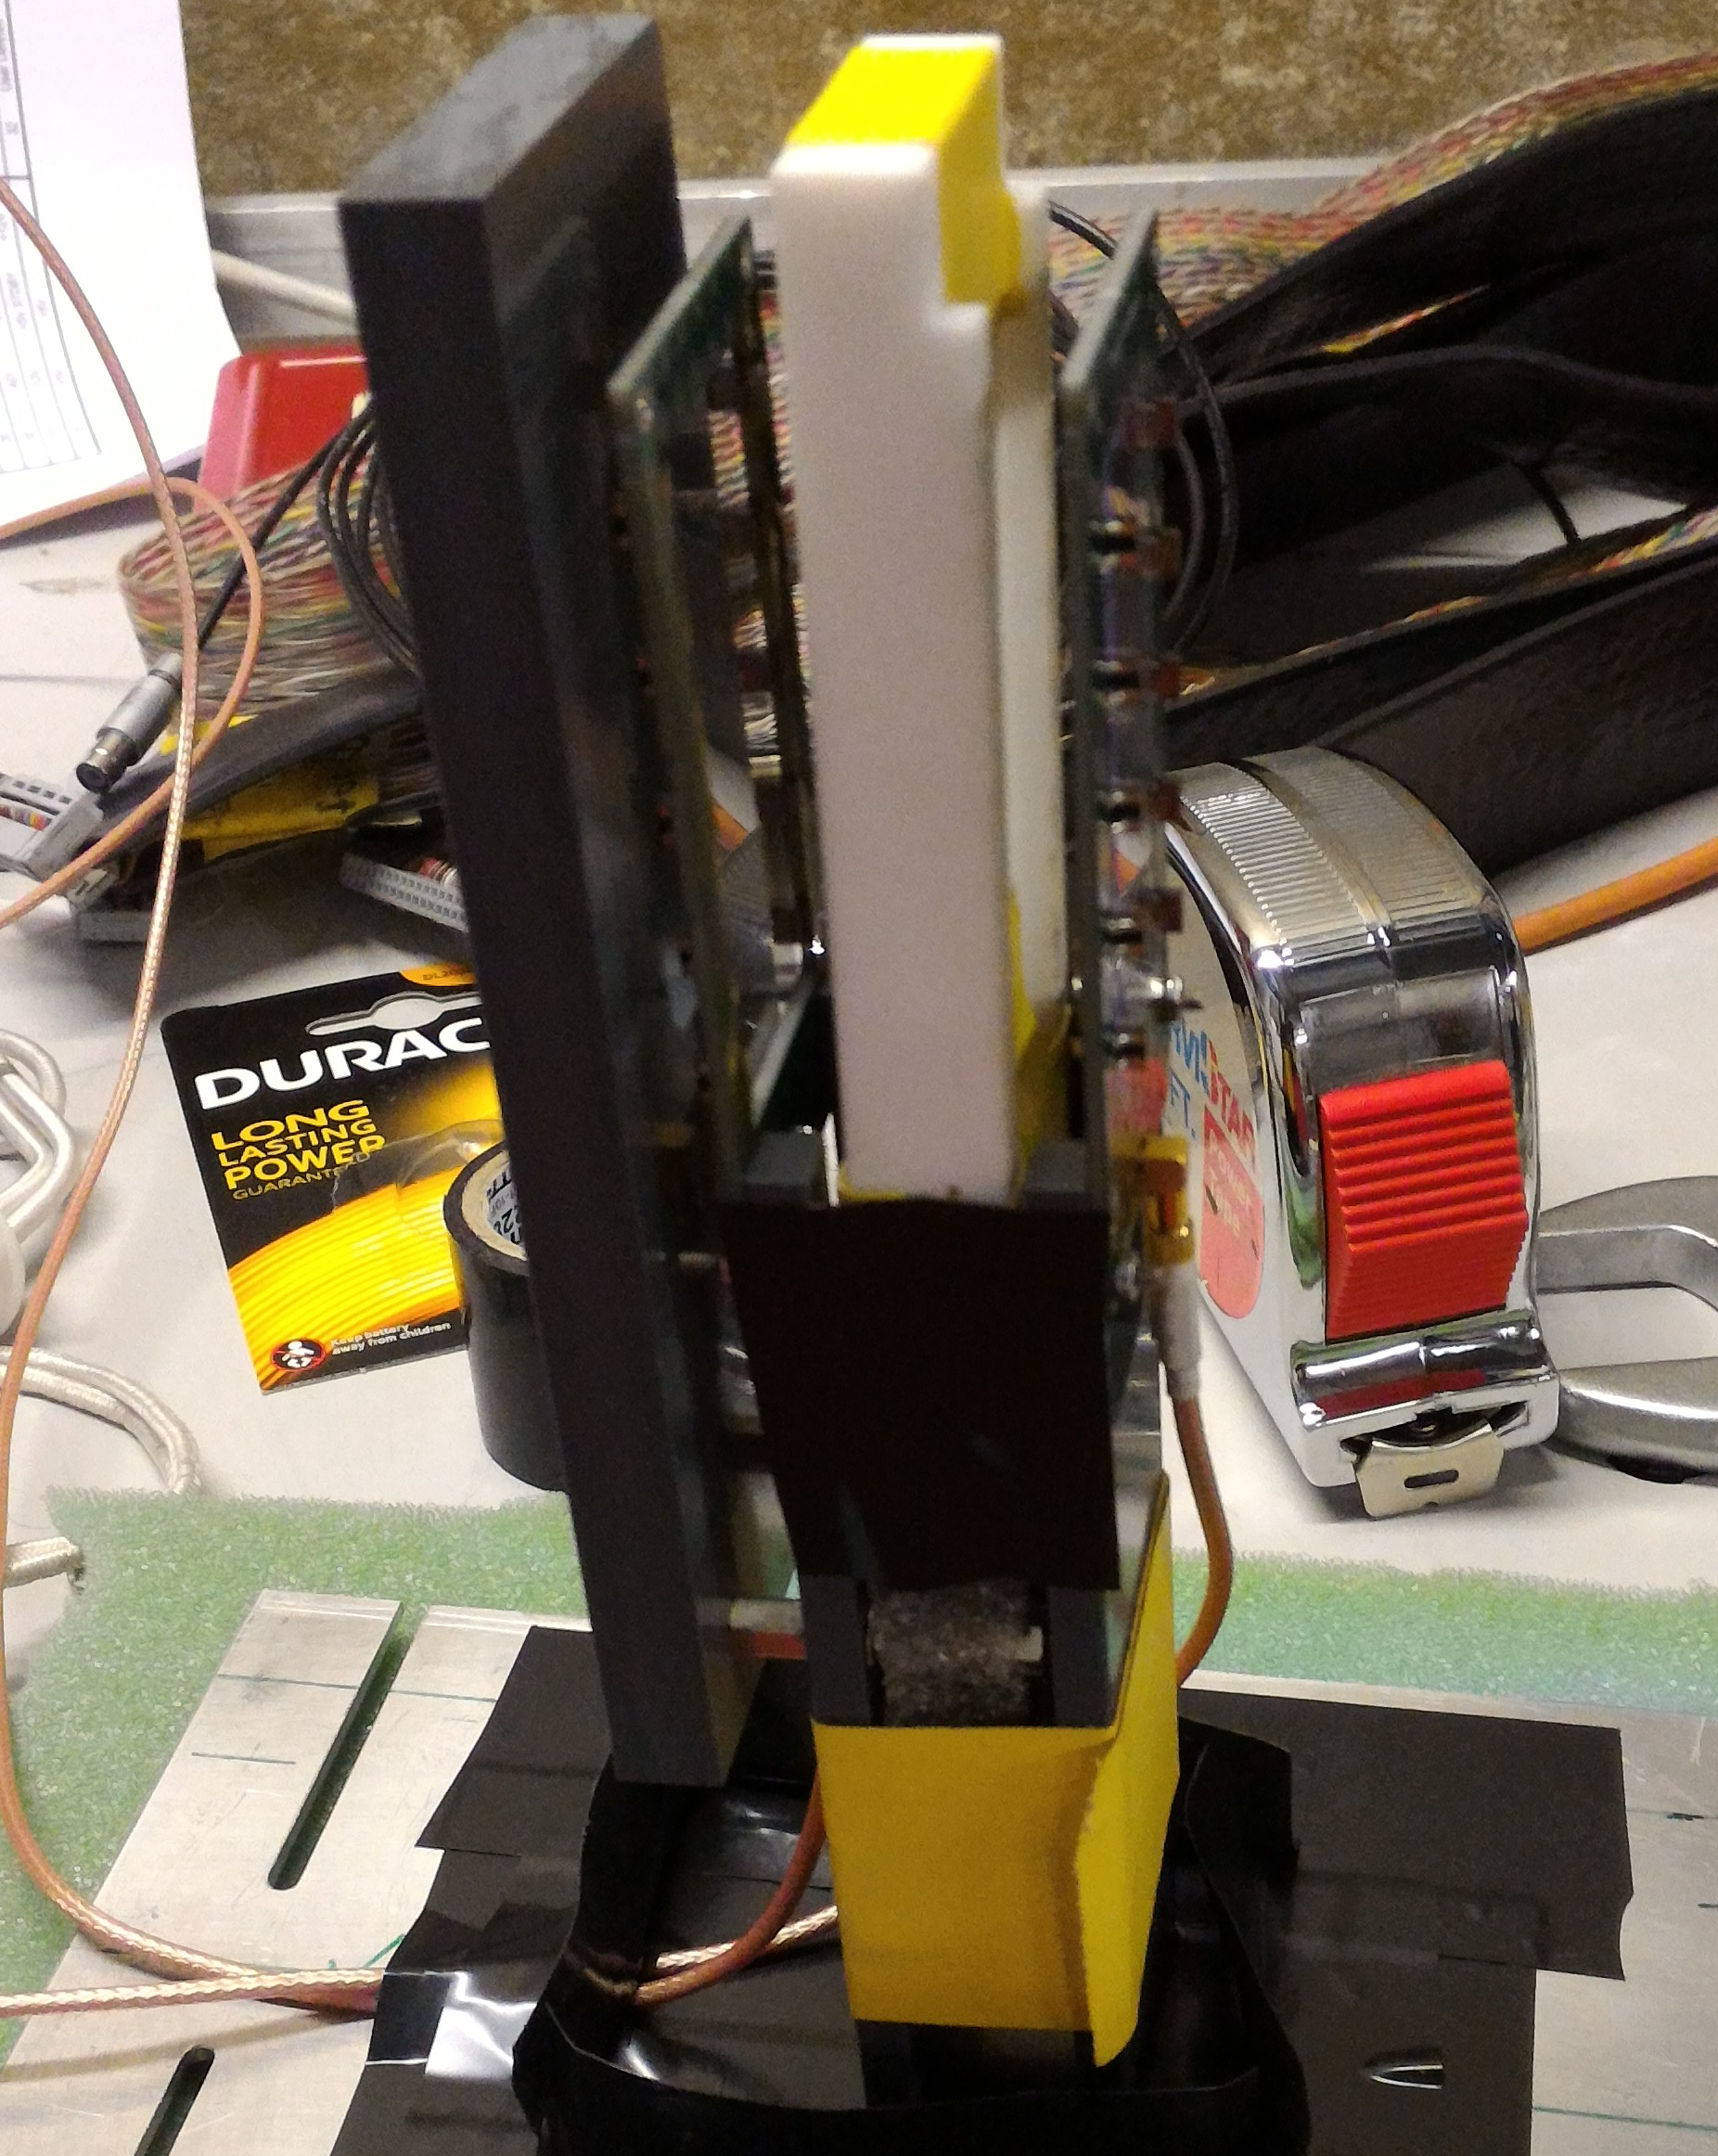
\includegraphics[width=0.49\textwidth]{neutrons/figures/R9Calib_Setup.jpg}
  \caption{Neutron wall stop calibration setup, with a block of macor as the target.}
  \label{fig:r9setup}
\end{figure}

By requiring a hit in the forward detector coincident with the muon entrance, we can select muons which predominantly stop in the target.
The rear detector serves as a veto to eliminate muons which punch through the targets, though for most targets this was not a major concern.
Testing was done with three of the primary construction materials for the TPC: silver, tungsten, and macor.
The resulting time distributions for electrons, neutrons and gammas are all shown in figure \ref{fig:r9_calib}, normalized by the number of events.
Testing was also performed with a spare TPC anode pad plane, which consists of a mixture of silver and tungsten.

\begin{figure}[h]
  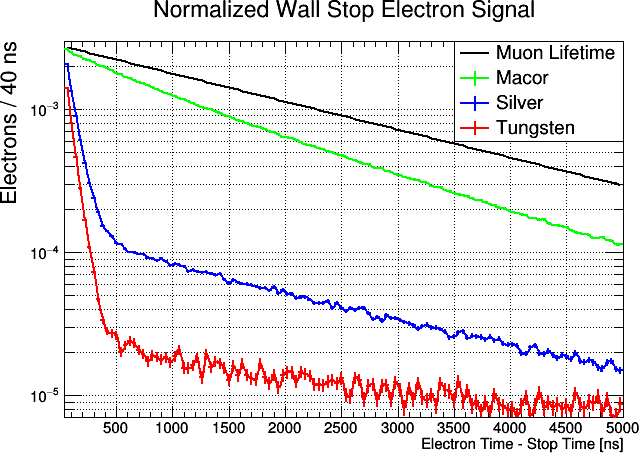
\includegraphics[width=0.49\textwidth]{neutrons/figures/R9Calib_Electron.png}
  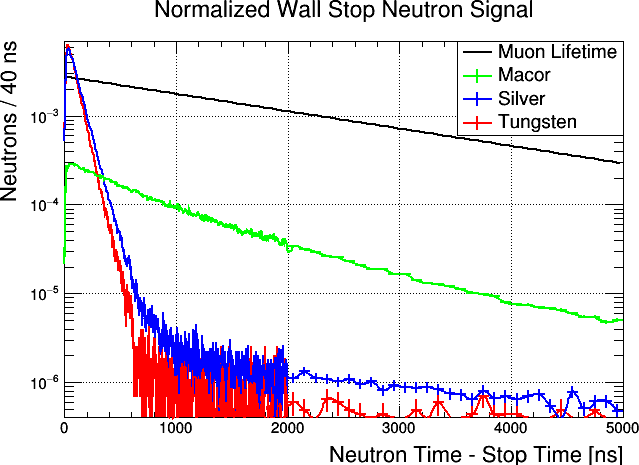
\includegraphics[width=0.49\textwidth]{neutrons/figures/R9Calib_Neutron.png} \\
  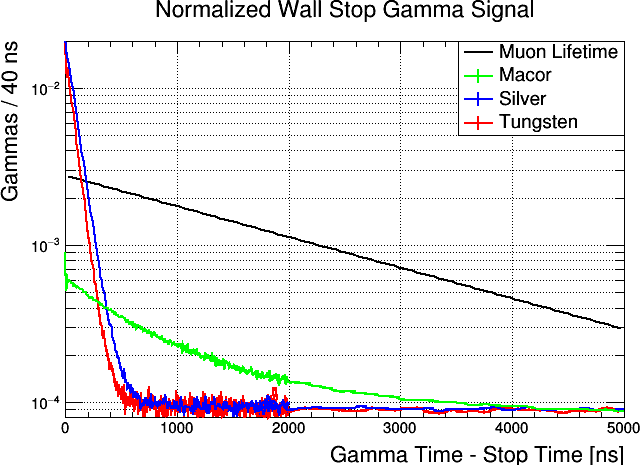
\includegraphics[width=0.49\textwidth]{neutrons/figures/R9Calib_Gamma.png}
  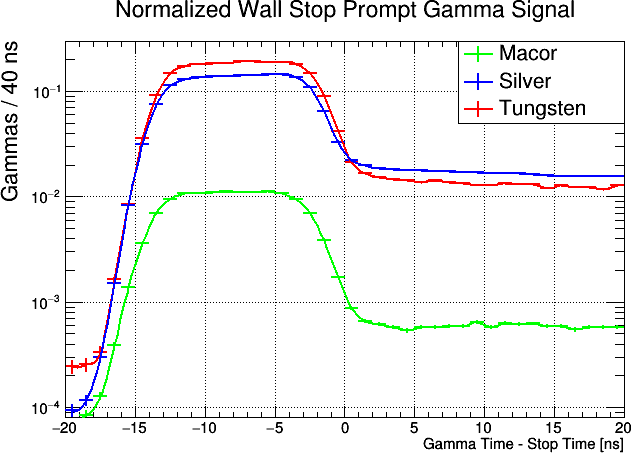
\includegraphics[width=0.49\textwidth]{neutrons/figures/R9Calib_Gamma2.png}
  \caption{Electron (1), Neutron (2), and Gamma (3) yields observed for various target materials, with an ideal muon decay curve shown for comparison.  Panel 4 shows a close-up of the gamma signal to show the prompt ACG signal.}
  \label{fig:r9calib}
\end{figure}

There are a few important features to note.  
First, for a pure wall stop signal we expect a single exponential decay, so the slow component of the observed time distributions must be due to muons which do not stop in the wall.  
The size of the slow electron component tells us the probability that a muon did not stop in the wall, which is slightly higher for silver since we used a thin foil target.
Second, we can see that the neutron signal is significantly larger than the electron signal despite the reduced solid angle coverage, and the gamma signal is larger still.
The background level for the neutrons is much lower though, making them the most sensitive signature of wall stops.
Finally, due to the low Z of the macor target the nuclear capture signal is much smaller and will be difficult to detect.
Macor still produces a distinctive ACG peak, albeit at relatively low energies, which allows for a loose limit on any macor stops.

While the 2016 calibrations allow us to convert the observed neutron detector signals to an absolute measure of the wall stops, there are complications due to differences in running conditions between the production runs.
In particular, the optimizations of the neutron digitizers in 2016 improved the PSD separation, altering the cut efficiency and allowing a lower minimum energy threshold for the neutrons.
There are also differences in the energy calibrations between the runs, and analysis of the 2014 data must take the difference in detectors into account.
To calibrate the wall stop signals, we must therefore examine the energy spectra.
Poor PSD separation results in a loss of efficiency at low energies while the smaller BICRON detectors lose efficiency at high energies, but we can match the spectra at intermediate energies.
The distinct peaks in the ACG energy spectra provide additional reference points for energy calibration and for evaluating the consistency of the observed signals.

\subsection{Results}

First, figure \ref{fig:scan_x} shows the results of an X scan, with fiducial volume cuts in the Y and Z axes.  
There do appear to be more wall stops in the boundary bins, presumably a combination of stops in the wires and of muons which continue traveling well past the point they exit the TPC.
The effect is relatively minor and there are few wall stops observed overall, as expected considering the relatively open boundaries of the TPC in the X direction.

\begin{figure}[h]
  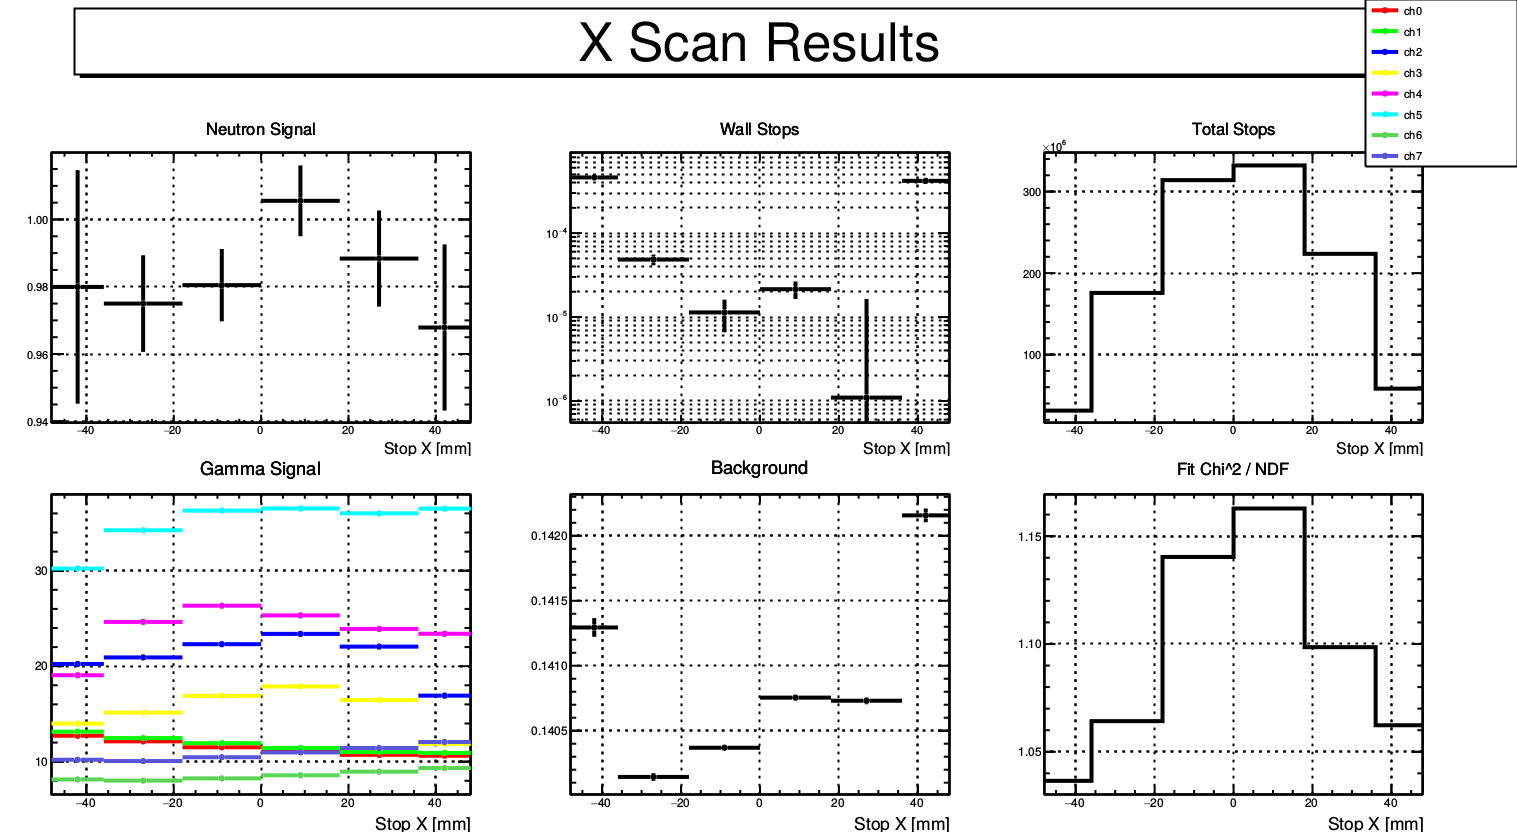
\includegraphics[width=\textwidth]{neutrons/figures/scan_X.png}
  \caption{Wall stop X scan.}
  \label{fig:scan_x}
\end{figure}

A two dimensional scan over the Y and Z axes is shown in figure \ref{fig:scan_yz}.
The individual one dimensional scans are somewhat misleading, as downstream stops tend to have shallower slopes resulting in more accurate estimates of the vertical stop position.
This effect produces a wall stop distribution which is broader for more upstream stops and gets narrower with increasing Z.
The results of this scan are used to define a relatively clean 'golden volume' for the purposes of the wall stop calibration.
The cuts we use are $3<Z<7$ and $20mm<Y<51mm$, omitting the first two Z pads and cutting $5mm$ from both directions in Y relative to the standard fiducial volume.

\begin{figure}[h]
  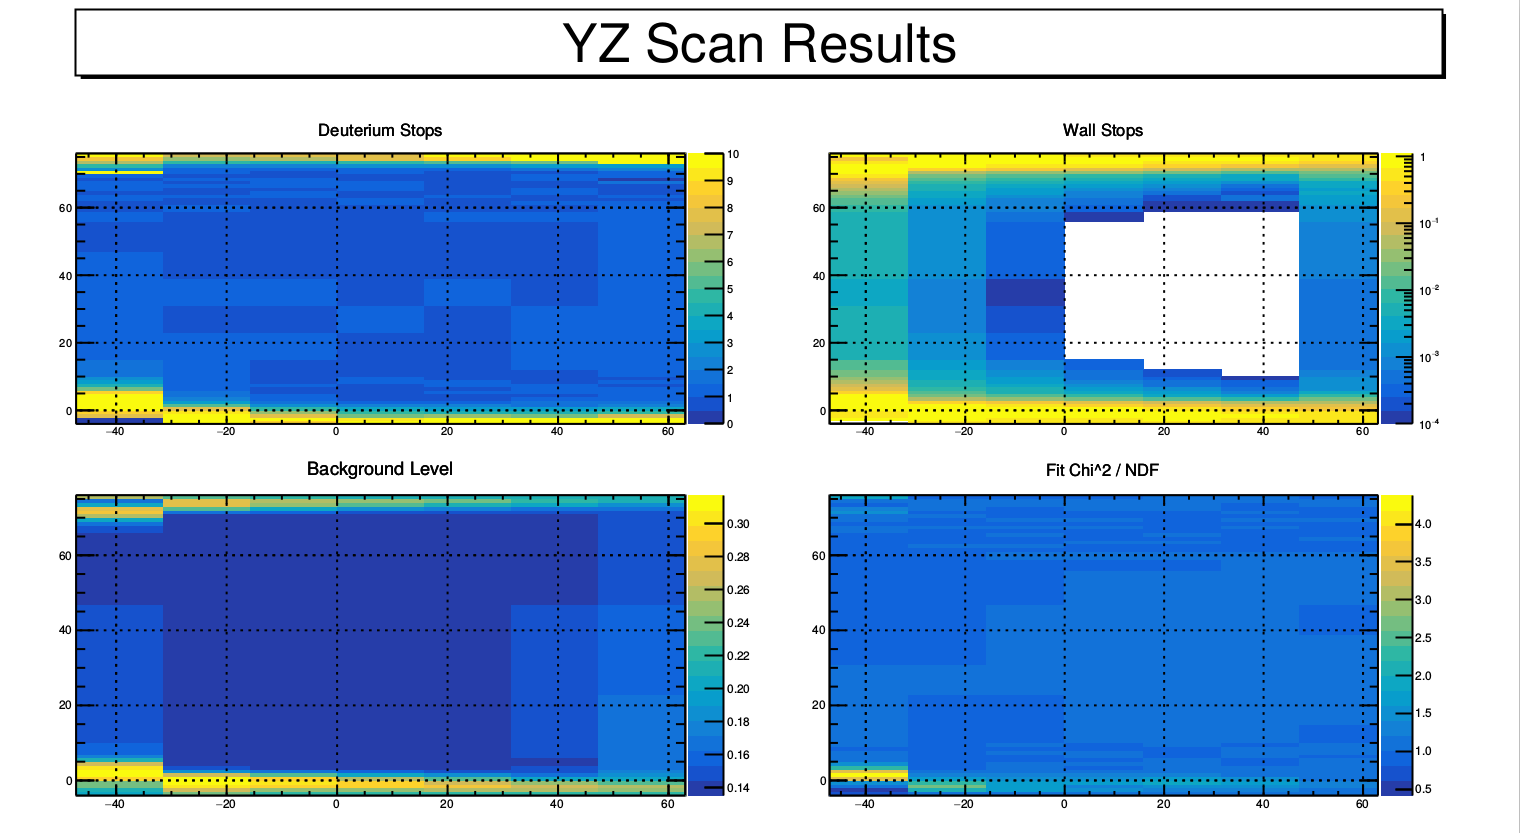
\includegraphics[width=\textwidth]{neutrons/figures/scan_YZ.png}
  \caption{Wall stop Y-Z scan.}
  \label{fig:scan_yz}
\end{figure}

Finally, we want to perform the fit in the fiducial volume to estimate our wall stop contamination.  
Using the golden volume defined above as our reference, we obtain a wall stop fraction in the fiducial volume of $(1.19 \pm 0.03) \times 10^{-4}$.

\subsection{Lifetime}

The effect of wall stops on our fitted muon lifetime depends greatly on the lifetime fit start time.  
Because stops in these high-Z materials rapidly capture, a small delay in the fit start time causes the number of remaining wall stops to drop drastically.
I wrote a simple script to simulate a lifetime fit with a given fraction $\alpha$ of wall stops.  
The resulting distribution is represented by a double exponential plus background:
\begin{equation}
f(t) = \frac{1-\alpha}{\lambda_{\mu}} e^{-\lambda_{\mu} t} + \frac{\alpha}{\lambda_{\mu}+\lambda_w} e^{-(\lambda_{\mu}+\lambda_w) t} + \epsilon_{BG}.
\end{equation}
This is fit with a single exponential plus background, with various start times and wall stop fractions.
The wall stop fractions in silver required to produce a $1 s^{-1}$ rate shift are shown in figure \ref{fig:lifetime_calib}.

\begin{figure}[h]
  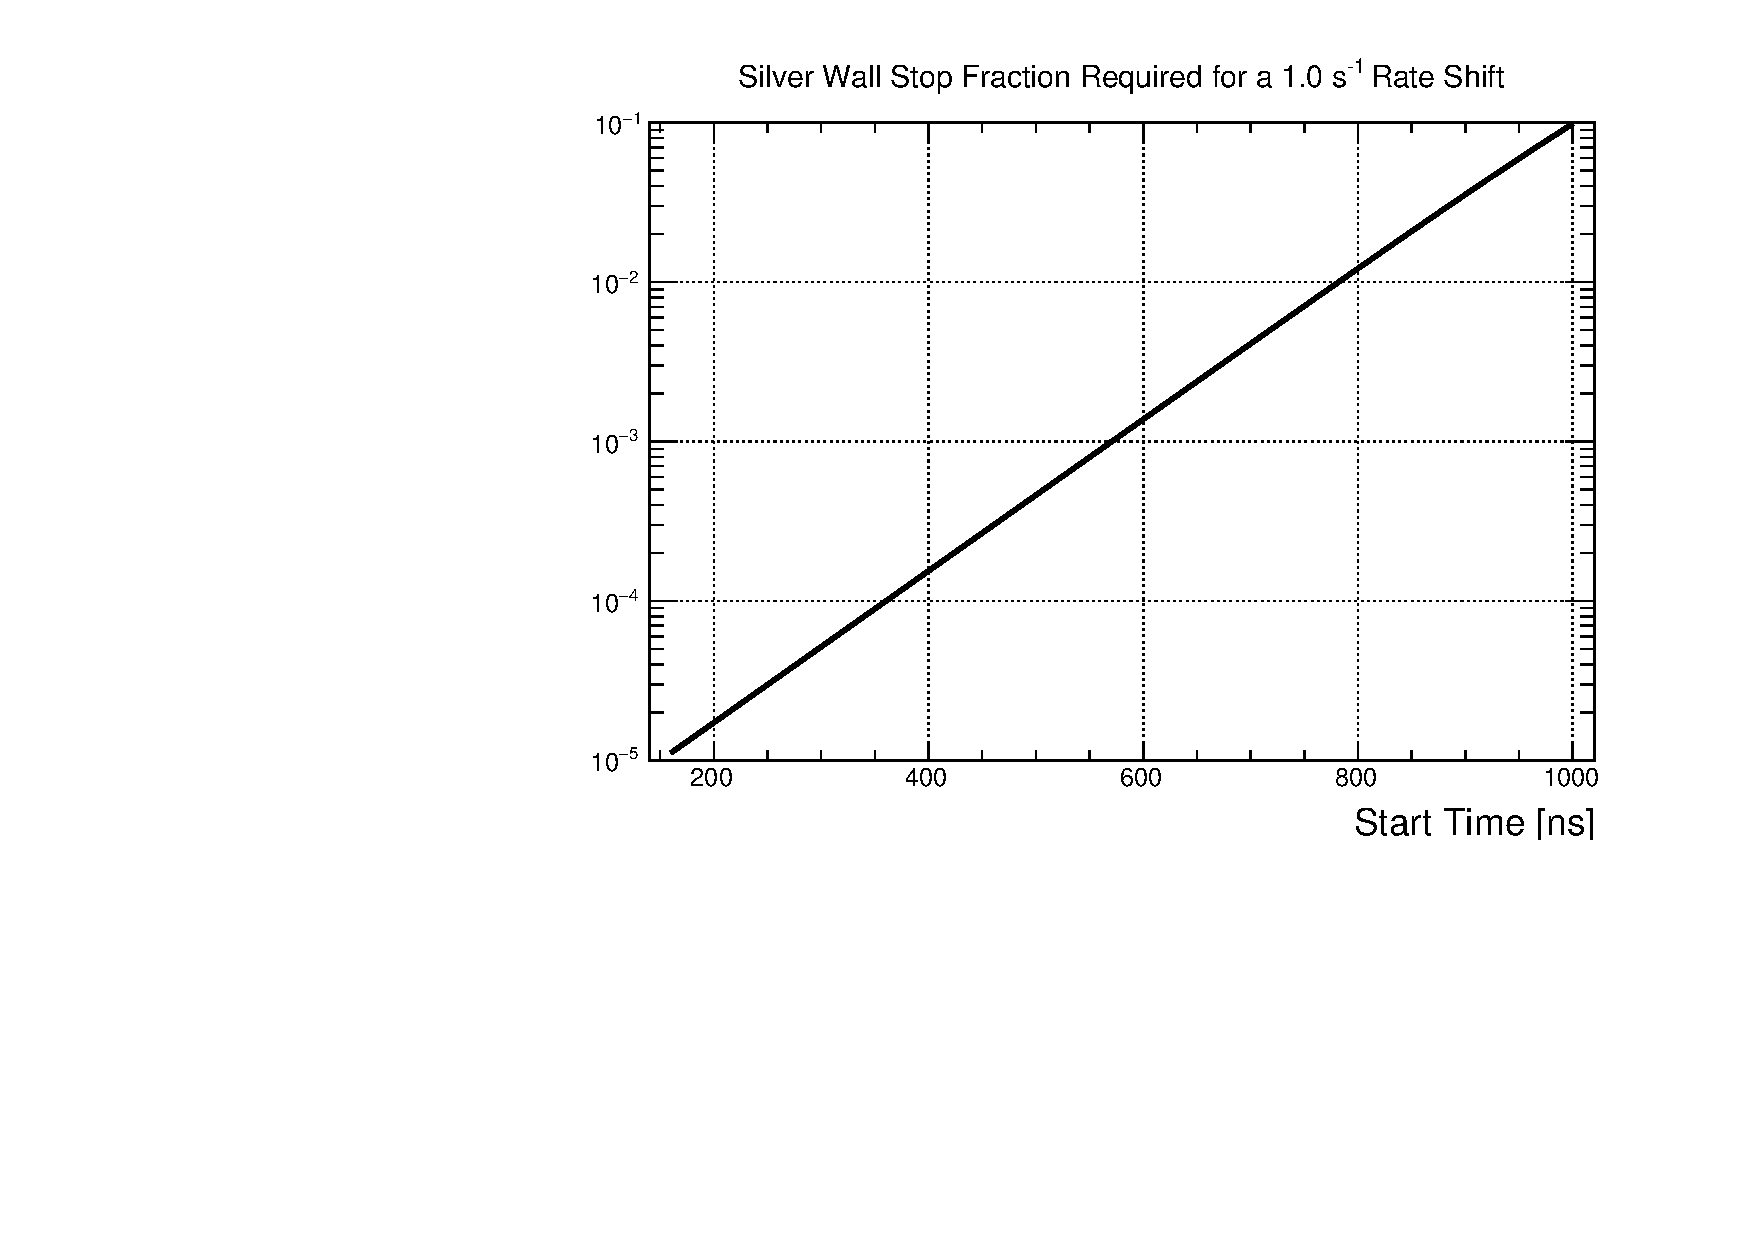
\includegraphics[width=\textwidth]{neutrons/figures/lifetime_calib.pdf}
  \caption{Estimated wall stop fraction required for a $1 s^{-1}$ rate shift, from simulation.}
  \label{fig:lifetime_calib}
\end{figure}

To avoid interference from the effect of the kicker on the background, most of our recent lifetime fits have been performed with a start time of $1 \mu s$.
In this case, we would require approximately 10\% wall stops to generate a $1 s^{-1}$ rate shift, and the $10^{-4}$ wall stop fraction in the fiducial volume is totally insignificant.  
Judging by the scans in the previous section, we could afford to omit the X and Z fiducial cuts, as well as expanding the fiducial volume in Y by around $10 mm$ in both directions.
Expansion of the fiducial volume requires more study, particularly on the effects of stops in diagonal bins which are not necessarily included in any of these scans. 
Nevertheless, this expansion could increase our statistics by up to nearly 60\%, allowing us to regain much of the loss due to the use of a later start time.

Alternatively, in the past we have sometimes used a start time of $160 ns$.  
In this case a $1 s^{-1}$ shift is produced with a wall stop fraction of only $1.11 \times 10^{-5}$.
The fiducial volume lifetime would therefore have a systematic error of $10.7 \pm 0.3 s^{-1}$.
At this point the correction is a bit large to simply apply after the fact, and it may be preferable to include the wall stop component in the lifetime fit model instead.  
Since we would need to use a more complicated lifetime fit to account for the time-dependent kicker backgrounds at these early times, the wall stops should be a straightforward addition.
Of course, if we are modeling the wall stops correctly in the lifetime fit then we may once again benefit from adjusting the fiducial volume as well.

